\documentclass[12pt,a4paper]{report}
% Unicode build: XeLaTeX or Tectonic. Times New Roman ships with Windows.
\usepackage{fontspec}
\setmainfont{Times New Roman}
\setsansfont{Arial}
\setmonofont{Consolas}[Scale=0.85]
\usepackage{amsmath,amssymb,amsfonts}
\usepackage{graphicx}
\usepackage{longtable}
\usepackage{hyperref}
\usepackage{geometry}
\geometry{a4paper, margin=2.5cm}
\hypersetup{unicode=true,hidelinks}
\emergencystretch=2em

\title{\textbf{BÁO CÁO TIỂU LUẬN DỰ ÁN}\\
\Large HỆ THỐNG TRUY XUẤT VĂN BẢN TIẾNG VIỆT SỬ DỤNG TF-IDF}
\author{Nhóm 7 -- Hệ cơ sở dữ liệu đa phương tiện}
\date{Ngày \number\day/\number\month/\number\year}

\begin{document}

\maketitle
\tableofcontents
\newpage

% Chương 1 — Giới thiệu. Được nạp bằng % Chương 1 — Giới thiệu. Được nạp bằng % Chương 1 — Giới thiệu. Được nạp bằng \input{chapter1} trong main.tex.
% Chỉ dùng các gói đã khai báo trong main.tex; không thêm gói mới.
\chapter{GIỚI THIỆU}

\section{Bối cảnh và lý do chọn đề tài}

Truy xuất văn bản là bài toán tìm trong một kho tài liệu những văn bản liên quan
nhất tới một câu hỏi của người dùng. Với tiếng Việt, bài toán này khó hơn so với
các ngôn ngữ dùng khoảng trắng để phân tách từ, vì khoảng trắng trong tiếng Việt
phân tách \emph{âm tiết} chứ không phân tách \emph{từ}: một từ như ``trí tuệ nhân
tạo'' gồm bốn âm tiết được viết rời nhau. Nếu lập chỉ mục trên từng âm tiết, các
âm tiết riêng lẻ như ``tuệ'' hay ``tạo'' trở thành đơn vị chỉ mục rời rạc và làm
loãng tín hiệu phân biệt của tài liệu. Vì vậy tách từ tiếng Việt là bước bắt buộc
trước khi biểu diễn và lập chỉ mục văn bản.

Một khó khăn thứ hai là lọc từ dừng. Loại các từ chức năng rất phổ biến (như
``của'', ``và'', ``là'') làm giảm nhiễu và kích thước chỉ mục, nhưng danh sách
cố định không tính đến đặc thù của từng miền dữ liệu. Trong kho tin tức tiếng
Việt theo nhiều chủ đề, có những từ phổ biến nhưng chỉ tập trung ở vài chủ đề;
loại chúng đi có thể làm mất thông tin phân biệt. Đề tài này tiếp cận bằng một
tầng lọc thứ hai dựa trên độ đo cấu trúc hình học chứ không dựa trên tần suất đặt
tay, nhằm trả lời câu hỏi: khi bỏ một từ khỏi không gian biểu diễn, các tài liệu
có trở nên dễ phân biệt nhau hơn hay không?

Đề tài được thực hiện trong phạm vi môn học đa phương tiện, với dữ liệu, thuật
toán và quy trình đo đều nằm lại trong kho mã nguồn của nhóm. Yêu cầu gốc của bài
tập nhóm bao gồm tách từ, loại từ dừng, biểu diễn TF-IDF, tính tương đồng cosin
và đánh giá kết quả \cite{baigiang}.

\section{Mục tiêu của đồ án}

Đồ án hướng tới các mục tiêu sau:

\begin{enumerate}
  \item Xây dựng một quy trình xử lý ngôn ngữ tiếng Việt hoàn chỉnh và có thể
        kiểm chứng: chuẩn hóa Unicode, tách từ theo ba phương pháp, và lọc từ
        dừng theo hai tầng.
  \item Cài đặt một hệ thống truy xuất văn bản trên nền TF-IDF và tương đồng
        cosin, có chỉ mục đảo, có khả năng giải thích điểm số theo từng từ.
  \item Cài đặt độ đo Giá trị phân biệt từ (Term Discrimination Value -- TDV)
        một cách chính xác để tự động phát hiện từ dừng đặc thù của miền dữ liệu.
  \item Bốn cấu hình thực nghiệm đối chứng (C1--C4) để so sánh các chiến lược
        lọc từ dừng trên cùng một kho ngữ liệu, cùng một bộ truy vấn và cùng một
        bộ nhãn liên quan.
  \item Đo độ trễ truy vấn và dung lượng chỉ mục bằng số liệu thật, có quy trình
        đo tách bạch khỏi các chỉ số chất lượng phụ thuộc nhãn người.
\end{enumerate}

\section{Phạm vi số liệu}

Kho ngữ liệu của đồ án gồm 2.500 bài báo tiếng Việt thuộc 10 lĩnh vực, mỗi lĩnh
vực 250 bài, được khóa bằng hàm băm SHA256 trong
\texttt{data/corpus\_manifest.json}. Bộ truy vấn gồm 20 câu, khoảng hai câu mỗi
lĩnh vực, phủ các dạng ngắn, dài, phủ định và chuyên ngành. Tập ứng viên đánh giá
được gộp từ kết quả của các đường cơ sở và được đưa cho người gán nhãn.

Một điểm được nêu rõ ngay từ đầu: báo cáo này \textbf{phân biệt rõ} giữa phần đã
đo và phần chưa đo. Trạng thái nhãn liên quan tại thời điểm viết là
\texttt{pending\_human\_annotation}: pool ứng viên đã hình thành nhưng \textbf{chưa
có cặp nào được người gán xác nhận}. Do đó các chỉ số chất lượng truy xuất
(P@K, R@K, F1@K, MAP, NDCG@K) \textbf{chưa được đo} và không được trình bày như
một kết quả đã có. Việc này là quyết định thiết kế: một bảng toàn số không khi
thiếu nhãn dễ bị đọc nhầm là hệ thống không tìm được gì, trong khi nguyên nhân là
thiếu dữ liệu gán nhãn.

\section{Yêu cầu của đề tài}

Theo yêu cầu bài tập nhóm \cite{baigiang}, sản phẩm cần thể hiện đủ ba phần lý
thuyết, cài đặt và thực nghiệm. Cụ thể đồ án phải có: (i) tách từ tiếng Việt bằng
\emph{so khớp cực đại} trên từ điển và cây Trie; (ii) loại từ dừng có nguồn và
quy tắc rõ ràng, không tự bù danh sách để đủ số lượng; (iii) biểu diễn văn bản và
truy vấn bằng TF-IDF, xếp hạng bằng tương đồng cosin; (iv) bộ công cụ đo lường và
biểu đồ kết quả. Nền tảng lý thuyết về biểu diễn văn bản và chỉ mục đảo được tham
chiếu từ giáo trình môn học \cite{giaotrinh}.

\section{Tổ chức thực hiện}

Công việc được chia thành ba nhóm trách nhiệm, ranh giới giữa các nhóm được ghi
thành hợp đồng API trong kho mã nguồn để tránh chồng lấn:

\begin{itemize}
  \item \textbf{M1 -- Xử lý ngôn ngữ tự nhiên:} chuẩn hóa chuỗi, từ điển và cây
        Trie, tách từ FMM/BMM/BiMM, lọc từ dừng tầng 1 cùng danh sách bảo vệ
        phủ định.
  \item \textbf{M2 -- Truy xuất thông tin:} TF-IDF, chỉ mục đảo, tương đồng
        cosin, độ đo TDV tầng 2, bộ đánh giá chỉ số và bộ đo độ trễ, dung lượng.
  \item \textbf{M3 -- Tích hợp và giao diện:} ứng dụng minh họa, hợp đồng API,
        quản trị mã nguồn và đóng gói.
\end{itemize}

Đồ án được thực hiện bởi Nhóm 7. Báo cáo dùng cách gọi nhất quán ``Nhóm 7'' trong
toàn bộ tài liệu.

\section{Đóng góp chính}

Các đóng góp được trình bày trong báo cáo gồm: một quy trình tách từ tiếng Việt
có vết thuật toán từng bước, tái lập được; một cài đặt TDV chính xác có đường
tham chiếu độc lập để kiểm chứng, kèm cả một phiên bản ``cách làm sai'' có chủ
đích để chứng minh rằng việc tái chuẩn hóa sau khi xóa một chiều là bắt buộc; một
bộ đánh giá có cổng chặn chống công bố kết quả giả khi thiếu nhãn hoặc sai hàm
băm; và một quy trình đo chất lượng tách từ bằng nhãn người với ràng buộc toàn vẹn
theo hàm băm.

\section{Cấu trúc báo cáo}

Phần còn lại của báo cáo được tổ chức như sau. Chương~2 trình bày nền tảng xử lý
ngôn ngữ tiếng Việt và lý do của từng bước tiền xử lý. Chương~3 trình bày thiết kế
hệ thống tìm kiếm, bao gồm thiết kế tầng ngôn ngữ M1, độ đo TF-IDF, độ đo TDV và
bốn cấu hình lọc. Chương~4 trình bày thực nghiệm và đánh giá. Chương~5 kết luận,
nêu rõ phần đã kiểm chứng và phần còn chờ nhãn người, cùng các hạn chế và hướng
phát triển.
 trong main.tex.
% Chỉ dùng các gói đã khai báo trong main.tex; không thêm gói mới.
\chapter{GIỚI THIỆU}

\section{Bối cảnh và lý do chọn đề tài}

Truy xuất văn bản là bài toán tìm trong một kho tài liệu những văn bản liên quan
nhất tới một câu hỏi của người dùng. Với tiếng Việt, bài toán này khó hơn so với
các ngôn ngữ dùng khoảng trắng để phân tách từ, vì khoảng trắng trong tiếng Việt
phân tách \emph{âm tiết} chứ không phân tách \emph{từ}: một từ như ``trí tuệ nhân
tạo'' gồm bốn âm tiết được viết rời nhau. Nếu lập chỉ mục trên từng âm tiết, các
âm tiết riêng lẻ như ``tuệ'' hay ``tạo'' trở thành đơn vị chỉ mục rời rạc và làm
loãng tín hiệu phân biệt của tài liệu. Vì vậy tách từ tiếng Việt là bước bắt buộc
trước khi biểu diễn và lập chỉ mục văn bản.

Một khó khăn thứ hai là lọc từ dừng. Loại các từ chức năng rất phổ biến (như
``của'', ``và'', ``là'') làm giảm nhiễu và kích thước chỉ mục, nhưng danh sách
cố định không tính đến đặc thù của từng miền dữ liệu. Trong kho tin tức tiếng
Việt theo nhiều chủ đề, có những từ phổ biến nhưng chỉ tập trung ở vài chủ đề;
loại chúng đi có thể làm mất thông tin phân biệt. Đề tài này tiếp cận bằng một
tầng lọc thứ hai dựa trên độ đo cấu trúc hình học chứ không dựa trên tần suất đặt
tay, nhằm trả lời câu hỏi: khi bỏ một từ khỏi không gian biểu diễn, các tài liệu
có trở nên dễ phân biệt nhau hơn hay không?

Đề tài được thực hiện trong phạm vi môn học đa phương tiện, với dữ liệu, thuật
toán và quy trình đo đều nằm lại trong kho mã nguồn của nhóm. Yêu cầu gốc của bài
tập nhóm bao gồm tách từ, loại từ dừng, biểu diễn TF-IDF, tính tương đồng cosin
và đánh giá kết quả \cite{baigiang}.

\section{Mục tiêu của đồ án}

Đồ án hướng tới các mục tiêu sau:

\begin{enumerate}
  \item Xây dựng một quy trình xử lý ngôn ngữ tiếng Việt hoàn chỉnh và có thể
        kiểm chứng: chuẩn hóa Unicode, tách từ theo ba phương pháp, và lọc từ
        dừng theo hai tầng.
  \item Cài đặt một hệ thống truy xuất văn bản trên nền TF-IDF và tương đồng
        cosin, có chỉ mục đảo, có khả năng giải thích điểm số theo từng từ.
  \item Cài đặt độ đo Giá trị phân biệt từ (Term Discrimination Value -- TDV)
        một cách chính xác để tự động phát hiện từ dừng đặc thù của miền dữ liệu.
  \item Bốn cấu hình thực nghiệm đối chứng (C1--C4) để so sánh các chiến lược
        lọc từ dừng trên cùng một kho ngữ liệu, cùng một bộ truy vấn và cùng một
        bộ nhãn liên quan.
  \item Đo độ trễ truy vấn và dung lượng chỉ mục bằng số liệu thật, có quy trình
        đo tách bạch khỏi các chỉ số chất lượng phụ thuộc nhãn người.
\end{enumerate}

\section{Phạm vi số liệu}

Kho ngữ liệu của đồ án gồm 2.500 bài báo tiếng Việt thuộc 10 lĩnh vực, mỗi lĩnh
vực 250 bài, được khóa bằng hàm băm SHA256 trong
\texttt{data/corpus\_manifest.json}. Bộ truy vấn gồm 20 câu, khoảng hai câu mỗi
lĩnh vực, phủ các dạng ngắn, dài, phủ định và chuyên ngành. Tập ứng viên đánh giá
được gộp từ kết quả của các đường cơ sở và được đưa cho người gán nhãn.

Một điểm được nêu rõ ngay từ đầu: báo cáo này \textbf{phân biệt rõ} giữa phần đã
đo và phần chưa đo. Trạng thái nhãn liên quan tại thời điểm viết là
\texttt{pending\_human\_annotation}: pool ứng viên đã hình thành nhưng \textbf{chưa
có cặp nào được người gán xác nhận}. Do đó các chỉ số chất lượng truy xuất
(P@K, R@K, F1@K, MAP, NDCG@K) \textbf{chưa được đo} và không được trình bày như
một kết quả đã có. Việc này là quyết định thiết kế: một bảng toàn số không khi
thiếu nhãn dễ bị đọc nhầm là hệ thống không tìm được gì, trong khi nguyên nhân là
thiếu dữ liệu gán nhãn.

\section{Yêu cầu của đề tài}

Theo yêu cầu bài tập nhóm \cite{baigiang}, sản phẩm cần thể hiện đủ ba phần lý
thuyết, cài đặt và thực nghiệm. Cụ thể đồ án phải có: (i) tách từ tiếng Việt bằng
\emph{so khớp cực đại} trên từ điển và cây Trie; (ii) loại từ dừng có nguồn và
quy tắc rõ ràng, không tự bù danh sách để đủ số lượng; (iii) biểu diễn văn bản và
truy vấn bằng TF-IDF, xếp hạng bằng tương đồng cosin; (iv) bộ công cụ đo lường và
biểu đồ kết quả. Nền tảng lý thuyết về biểu diễn văn bản và chỉ mục đảo được tham
chiếu từ giáo trình môn học \cite{giaotrinh}.

\section{Tổ chức thực hiện}

Công việc được chia thành ba nhóm trách nhiệm, ranh giới giữa các nhóm được ghi
thành hợp đồng API trong kho mã nguồn để tránh chồng lấn:

\begin{itemize}
  \item \textbf{M1 -- Xử lý ngôn ngữ tự nhiên:} chuẩn hóa chuỗi, từ điển và cây
        Trie, tách từ FMM/BMM/BiMM, lọc từ dừng tầng 1 cùng danh sách bảo vệ
        phủ định.
  \item \textbf{M2 -- Truy xuất thông tin:} TF-IDF, chỉ mục đảo, tương đồng
        cosin, độ đo TDV tầng 2, bộ đánh giá chỉ số và bộ đo độ trễ, dung lượng.
  \item \textbf{M3 -- Tích hợp và giao diện:} ứng dụng minh họa, hợp đồng API,
        quản trị mã nguồn và đóng gói.
\end{itemize}

Đồ án được thực hiện bởi Nhóm 7. Báo cáo dùng cách gọi nhất quán ``Nhóm 7'' trong
toàn bộ tài liệu.

\section{Đóng góp chính}

Các đóng góp được trình bày trong báo cáo gồm: một quy trình tách từ tiếng Việt
có vết thuật toán từng bước, tái lập được; một cài đặt TDV chính xác có đường
tham chiếu độc lập để kiểm chứng, kèm cả một phiên bản ``cách làm sai'' có chủ
đích để chứng minh rằng việc tái chuẩn hóa sau khi xóa một chiều là bắt buộc; một
bộ đánh giá có cổng chặn chống công bố kết quả giả khi thiếu nhãn hoặc sai hàm
băm; và một quy trình đo chất lượng tách từ bằng nhãn người với ràng buộc toàn vẹn
theo hàm băm.

\section{Cấu trúc báo cáo}

Phần còn lại của báo cáo được tổ chức như sau. Chương~2 trình bày nền tảng xử lý
ngôn ngữ tiếng Việt và lý do của từng bước tiền xử lý. Chương~3 trình bày thiết kế
hệ thống tìm kiếm, bao gồm thiết kế tầng ngôn ngữ M1, độ đo TF-IDF, độ đo TDV và
bốn cấu hình lọc. Chương~4 trình bày thực nghiệm và đánh giá. Chương~5 kết luận,
nêu rõ phần đã kiểm chứng và phần còn chờ nhãn người, cùng các hạn chế và hướng
phát triển.
 trong main.tex.
% Chỉ dùng các gói đã khai báo trong main.tex; không thêm gói mới.
\chapter{GIỚI THIỆU}

\section{Bối cảnh và lý do chọn đề tài}

Truy xuất văn bản là bài toán tìm trong một kho tài liệu những văn bản liên quan
nhất tới một câu hỏi của người dùng. Với tiếng Việt, bài toán này khó hơn so với
các ngôn ngữ dùng khoảng trắng để phân tách từ, vì khoảng trắng trong tiếng Việt
phân tách \emph{âm tiết} chứ không phân tách \emph{từ}: một từ như ``trí tuệ nhân
tạo'' gồm bốn âm tiết được viết rời nhau. Nếu lập chỉ mục trên từng âm tiết, các
âm tiết riêng lẻ như ``tuệ'' hay ``tạo'' trở thành đơn vị chỉ mục rời rạc và làm
loãng tín hiệu phân biệt của tài liệu. Vì vậy tách từ tiếng Việt là bước bắt buộc
trước khi biểu diễn và lập chỉ mục văn bản.

Một khó khăn thứ hai là lọc từ dừng. Loại các từ chức năng rất phổ biến (như
``của'', ``và'', ``là'') làm giảm nhiễu và kích thước chỉ mục, nhưng danh sách
cố định không tính đến đặc thù của từng miền dữ liệu. Trong kho tin tức tiếng
Việt theo nhiều chủ đề, có những từ phổ biến nhưng chỉ tập trung ở vài chủ đề;
loại chúng đi có thể làm mất thông tin phân biệt. Đề tài này tiếp cận bằng một
tầng lọc thứ hai dựa trên độ đo cấu trúc hình học chứ không dựa trên tần suất đặt
tay, nhằm trả lời câu hỏi: khi bỏ một từ khỏi không gian biểu diễn, các tài liệu
có trở nên dễ phân biệt nhau hơn hay không?

Đề tài được thực hiện trong phạm vi môn học đa phương tiện, với dữ liệu, thuật
toán và quy trình đo đều nằm lại trong kho mã nguồn của nhóm. Yêu cầu gốc của bài
tập nhóm bao gồm tách từ, loại từ dừng, biểu diễn TF-IDF, tính tương đồng cosin
và đánh giá kết quả \cite{baigiang}.

\section{Mục tiêu của đồ án}

Đồ án hướng tới các mục tiêu sau:

\begin{enumerate}
  \item Xây dựng một quy trình xử lý ngôn ngữ tiếng Việt hoàn chỉnh và có thể
        kiểm chứng: chuẩn hóa Unicode, tách từ theo ba phương pháp, và lọc từ
        dừng theo hai tầng.
  \item Cài đặt một hệ thống truy xuất văn bản trên nền TF-IDF và tương đồng
        cosin, có chỉ mục đảo, có khả năng giải thích điểm số theo từng từ.
  \item Cài đặt độ đo Giá trị phân biệt từ (Term Discrimination Value -- TDV)
        một cách chính xác để tự động phát hiện từ dừng đặc thù của miền dữ liệu.
  \item Bốn cấu hình thực nghiệm đối chứng (C1--C4) để so sánh các chiến lược
        lọc từ dừng trên cùng một kho ngữ liệu, cùng một bộ truy vấn và cùng một
        bộ nhãn liên quan.
  \item Đo độ trễ truy vấn và dung lượng chỉ mục bằng số liệu thật, có quy trình
        đo tách bạch khỏi các chỉ số chất lượng phụ thuộc nhãn người.
\end{enumerate}

\section{Phạm vi số liệu}

Kho ngữ liệu của đồ án gồm 2.500 bài báo tiếng Việt thuộc 10 lĩnh vực, mỗi lĩnh
vực 250 bài, được khóa bằng hàm băm SHA256 trong
\texttt{data/corpus\_manifest.json}. Bộ truy vấn gồm 20 câu, khoảng hai câu mỗi
lĩnh vực, phủ các dạng ngắn, dài, phủ định và chuyên ngành. Tập ứng viên đánh giá
được gộp từ kết quả của các đường cơ sở và được đưa cho người gán nhãn.

Một điểm được nêu rõ ngay từ đầu: báo cáo này \textbf{phân biệt rõ} giữa phần đã
đo và phần chưa đo. Trạng thái nhãn liên quan tại thời điểm viết là
\texttt{pending\_human\_annotation}: pool ứng viên đã hình thành nhưng \textbf{chưa
có cặp nào được người gán xác nhận}. Do đó các chỉ số chất lượng truy xuất
(P@K, R@K, F1@K, MAP, NDCG@K) \textbf{chưa được đo} và không được trình bày như
một kết quả đã có. Việc này là quyết định thiết kế: một bảng toàn số không khi
thiếu nhãn dễ bị đọc nhầm là hệ thống không tìm được gì, trong khi nguyên nhân là
thiếu dữ liệu gán nhãn.

\section{Yêu cầu của đề tài}

Theo yêu cầu bài tập nhóm \cite{baigiang}, sản phẩm cần thể hiện đủ ba phần lý
thuyết, cài đặt và thực nghiệm. Cụ thể đồ án phải có: (i) tách từ tiếng Việt bằng
\emph{so khớp cực đại} trên từ điển và cây Trie; (ii) loại từ dừng có nguồn và
quy tắc rõ ràng, không tự bù danh sách để đủ số lượng; (iii) biểu diễn văn bản và
truy vấn bằng TF-IDF, xếp hạng bằng tương đồng cosin; (iv) bộ công cụ đo lường và
biểu đồ kết quả. Nền tảng lý thuyết về biểu diễn văn bản và chỉ mục đảo được tham
chiếu từ giáo trình môn học \cite{giaotrinh}.

\section{Tổ chức thực hiện}

Công việc được chia thành ba nhóm trách nhiệm, ranh giới giữa các nhóm được ghi
thành hợp đồng API trong kho mã nguồn để tránh chồng lấn:

\begin{itemize}
  \item \textbf{M1 -- Xử lý ngôn ngữ tự nhiên:} chuẩn hóa chuỗi, từ điển và cây
        Trie, tách từ FMM/BMM/BiMM, lọc từ dừng tầng 1 cùng danh sách bảo vệ
        phủ định.
  \item \textbf{M2 -- Truy xuất thông tin:} TF-IDF, chỉ mục đảo, tương đồng
        cosin, độ đo TDV tầng 2, bộ đánh giá chỉ số và bộ đo độ trễ, dung lượng.
  \item \textbf{M3 -- Tích hợp và giao diện:} ứng dụng minh họa, hợp đồng API,
        quản trị mã nguồn và đóng gói.
\end{itemize}

Đồ án được thực hiện bởi Nhóm 7. Báo cáo dùng cách gọi nhất quán ``Nhóm 7'' trong
toàn bộ tài liệu.

\section{Đóng góp chính}

Các đóng góp được trình bày trong báo cáo gồm: một quy trình tách từ tiếng Việt
có vết thuật toán từng bước, tái lập được; một cài đặt TDV chính xác có đường
tham chiếu độc lập để kiểm chứng, kèm cả một phiên bản ``cách làm sai'' có chủ
đích để chứng minh rằng việc tái chuẩn hóa sau khi xóa một chiều là bắt buộc; một
bộ đánh giá có cổng chặn chống công bố kết quả giả khi thiếu nhãn hoặc sai hàm
băm; và một quy trình đo chất lượng tách từ bằng nhãn người với ràng buộc toàn vẹn
theo hàm băm.

\section{Cấu trúc báo cáo}

Phần còn lại của báo cáo được tổ chức như sau. Chương~2 trình bày nền tảng xử lý
ngôn ngữ tiếng Việt và lý do của từng bước tiền xử lý. Chương~3 trình bày thiết kế
hệ thống tìm kiếm, bao gồm thiết kế tầng ngôn ngữ M1, độ đo TF-IDF, độ đo TDV và
bốn cấu hình lọc. Chương~4 trình bày thực nghiệm và đánh giá. Chương~5 kết luận,
nêu rõ phần đã kiểm chứng và phần còn chờ nhãn người, cùng các hạn chế và hướng
phát triển.


% Chương 2 — Nền tảng xử lý ngôn ngữ tiếng Việt. Nạp bằng % Chương 2 — Nền tảng xử lý ngôn ngữ tiếng Việt. Nạp bằng % Chương 2 — Nền tảng xử lý ngôn ngữ tiếng Việt. Nạp bằng \input{chapter2_nlp}.
% Chỉ dùng các gói đã khai báo trong main.tex; không thêm gói mới.
\chapter{NỀN TẢNG XỬ LÝ NGÔN NGỮ TIẾNG VIỆT}
\label{ch:ch2-nlp}

Chương này trình bày các khái niệm ngôn ngữ học và các quyết định tiền xử lý mà
hệ thống dựa vào. Mục tiêu không phải trình bày lý thuyết ngôn ngữ học đầy đủ, mà
là chỉ ra chính xác vì sao mỗi bước trong quy trình tiền xử lý tồn tại và nó ảnh
hưởng gì tới kết quả truy xuất.

\section{Âm tiết và từ trong tiếng Việt}

Tiếng Việt là ngôn ngữ đơn lập và có thanh điệu. Đơn vị ngữ âm cơ bản là
\emph{âm tiết}; trong chữ Quốc ngữ, các âm tiết được viết rời nhau bằng khoảng
trắng. Tuy nhiên đơn vị mang nghĩa dùng cho truy xuất lại là \emph{từ}, và một từ
thường gồm nhiều âm tiết. Ví dụ, ``trí tuệ nhân tạo'' là một cụm bốn âm tiết gắn
với một khái niệm, ``giáo dục'' là một từ hai âm tiết. Ranh giới từ không hiển
thị trực tiếp trên văn bản, nên cần một bộ tách từ để phục hồi ranh giới đó.

Sự lệch pha giữa cách viết (khoảng trắng) và đơn vị nghĩa (từ) là cái bẫy lớn
nhất khi lập chỉ mục tiếng Việt. Nếu coi mỗi âm tiết là một đơn vị chỉ mục, thì
``trí'', ``tuệ'', ``nhân'', ``tạo'' trở thành bốn chiều tách rời; khái niệm
``trí tuệ nhân tạo'' bị phân rã và tín hiệu phân biệt bị pha loãng bởi các âm tiết
rất phổ biến. Đây là lý do bước tách từ được đặt trước bước lập chỉ mục.

\section{Chuẩn hóa Unicode và dấu thanh}

Tiếng Việt dùng nhiều dấu thanh và dấu mũ, và cùng một chữ có thể được mã hóa theo
hai cách trong Unicode: dạng tổ hợp (một chữ cái cơ bản cộng dấu tổ hợp) và dạng
dựng sẵn (một điểm mã duy nhất). Hai chuỗi trông giống hệt nhau trên màn hình
nhưng khác nhau về dãy điểm mã sẽ không khớp nhau khi so sánh, khi tra từ điển
hay khi tính hàm băm. Vì vậy toàn bộ văn bản được chuẩn hóa về dạng dựng sẵn
Unicode NFC trước khi xử lý tiếp.

Bên cạnh chuẩn hóa tổ hợp dấu, quy trình còn hạ chữ hoa xuống chữ thường và loại
bỏ các thành phần không mang nội dung như thẻ đánh dấu, đường dẫn và địa chỉ thư
điện tử. Chi tiết các quy tắc này cùng lý do của từng quy tắc được trình bày ở
Chương~3, phần thiết kế tầng ngôn ngữ M1.

\section{Vì sao phải tách từ trước khi lập chỉ mục}

Biểu diễn túi từ (bag of words) bỏ qua thứ tự từ và coi mỗi đơn vị chỉ mục là một
chiều độc lập. Với ngôn ngữ dùng khoảng trắng phân tách từ, đơn vị đó là từ. Với
tiếng Việt, phải chủ động tạo ra đơn vị đó bằng tách từ. Tách từ đúng làm cho
``giáo dục'' là một chiều thay vì hai, và làm cho ``trí tuệ nhân tạo'' là một chiều
thay vì bốn. Cách làm này vừa giảm số chiều hiệu dụng, vừa tăng khả năng phân biệt
của các chiều còn lại.

Ngược lại, tách sai gây hại kép. Ghép nhầm hai đơn vị vốn độc lập làm mất một
chiều có nghĩa; cắt rời một từ ghép làm mất một chiều có nghĩa khác. Vì vậy tách
từ là bước cần được đo chất lượng bằng nhãn người chứ không chỉ bằng các ca kiểm
thử nhỏ.

\section{So khớp cực đại: FMM, BMM và BiMM}

Hướng tiếp cận được nhóm chọn là so khớp cực đại dựa trên từ điển, hoạt động hoàn
toàn ngoại tuyến và có vết thuật toán từng bước để kiểm chứng. Ý tưởng chung là
trượt một cửa sổ gồm tối đa $L$ âm tiết trên câu đã chuẩn hóa và chọn đoạn dài
nhất có mặt trong từ điển.

\begin{itemize}
  \item \textbf{FMM (so khớp tiến cực đại):} duyệt câu từ trái sang phải; tại mỗi
        vị trí, thử cửa sổ dài nhất rồi rút ngắn dần cho đến khi gặp một đoạn có
        trong từ điển.
  \item \textbf{BMM (so khớp lùi cực đại):} làm tương tự nhưng duyệt từ phải sang
        trái.
  \item \textbf{BiMM (so khớp hai chiều):} chạy cả hai hướng rồi chọn kết quả theo
        một bộ quy tắc phân xử.
\end{itemize}

Nhập nhằng là đặc trưng của phương pháp này. Với câu ``học sinh học sinh học'',
cả ``học sinh'' và ``sinh học'' đều là từ hợp lệ trong từ điển, nên FMM và BMM có
thể cho hai cách tách khác nhau trên cùng một câu. Bộ quy tắc phân xử của BiMM vì
vậy được định nghĩa theo thứ tự ưu tiên rõ ràng: chọn phương án có ít đơn vị hơn,
rồi ít âm tiết đơn hơn, rồi ít đơn vị ngoài từ điển hơn, và khi tất cả đều hòa thì
chọn BMM. Quy tắc này và cách kiểm chứng bằng từ điển fixture minh bạch được trình
bày ở Chương~3.

\section{Từ dừng, phủ định và bài toán lọc hai tầng}

Từ dừng là các từ chức năng xuất hiện rất phổ biến nhưng đóng góp ít cho việc phân
biệt tài liệu. Loại chúng đi giúp tăng trọng số tương đối của các từ mang nội dung
và giảm kích thước chỉ mục. Tuy nhiên có hai cạm bẫy.

Thứ nhất, một danh sách từ dừng cố định không tính đến miền dữ liệu. Từ rất phổ
biến trong kho tin tức thể thao có thể là từ hiếm và có giá trị trong một kho y
tế; ngược lại, có từ phổ biến chung nhưng lại tập trung ở vài chủ đề và mang
thông tin phân biệt. Vì vậy đồ án dùng hai tầng: tầng~1 loại hư từ ngữ pháp bằng
danh sách có nguồn và quy tắc biên soạn; tầng~2 dùng độ đo hình học TDV để phát
hiện từ dừng đặc thù của chính miền dữ liệu.

Thứ hai, phủ định mang thông tin điều kiện chân trị. Trong truy vấn ``bệnh không
truyền nhiễm'', ``không'' làm đảo nghĩa của cả cụm; loại ``không'' đi thì truy vấn
còn lại nói về ``bệnh truyền nhiễm'' -- nghĩa gần như ngược lại. Vì vậy theo sau
tầng lọc phải có một danh sách bảo vệ (guard) gỡ lại các từ phủ định và logic.
Đồ án giữ quy tắc: một từ được bảo vệ nếu chính nó nằm trong danh sách guard, hoặc
nếu một thành phần trong từ ghép của nó là guard được bảo vệ, nhờ đó các từ ghép
như ``không thể'' cũng được giữ nguyên vẹn.

Cần nói rõ giới hạn: giữ lại từ phủ định trong túi từ không biến mô hình thành bộ
suy luận phủ định theo ngữ nghĩa. Túi từ vẫn chỉ ghi nhận sự xuất hiện của từ
``không'', chứ không suy ra được quan hệ điều kiện chân trị phức tạp. Việc bảo vệ
guard chỉ ngăn chặn việc lọc làm mất dấu hiệu phủ định ở mức từ vựng.

\section{Từ điển tiếng Việt sử dụng}

Bước tách từ dựa trên một từ điển tiếng Việt đóng gói trong kho mã nguồn. Nhóm sử
dụng danh sách Viet74K \cite{viet74k}, một danh sách từ tiếng Việt mã nguồn mở,
được ghim ở một phiên bản (commit) cụ thể và đi kèm thông tin giấy phép. Từ điển
gồm 69.858 mục sau khi làm sạch; độ dài tối đa là 17 âm tiết, và khoảng 97,42\%
số mục có không quá bốn âm tiết. Con số độ dài tối đa dùng để đặt cửa sổ trượt
$L$ sao cho không bỏ sót mục nào, còn phân bố độ dài cho thấy phần lớn từ có độ
dài ngắn.

Đi kèm từ điển là một tệp thống kê mô tả số mục, phân bố độ dài và hàm băm của
tệp từ điển, để bất kỳ ai cũng có thể kiểm tra lại dữ liệu đã dùng. Chất lượng
tách từ phụ thuộc từ điển: đổi từ điển thì mọi số đo tách từ phải được đo lại, vì
cùng một câu có thể được tách khác đi.

\section{Từ vựng đến vector đặc trưng}

Sau tách từ và lọc từ dừng, mỗi tài liệu được biểu diễn thành một vector trọng số
trên từ vựng chung. Chương~3 trình bày công thức trọng số TF-IDF, cách chuẩn hóa
vector và cách tính tương đồng cosin. Trọng số không phải là số đếm thô: nó kết
hợp tần suất trong tài liệu với độ hiếm của từ trên toàn kho, nhờ đó các từ hiếm
nhưng phân biệt được đề cao hơn các từ phổ biến. Đây cũng là trực giác dẫn tới
tầng lọc thứ hai bằng TDV, bởi TDV đo trực tiếp tác động của việc bỏ một từ lên
khả năng phân biệt tài liệu, thay vì gián tiếp qua tần suất.
.
% Chỉ dùng các gói đã khai báo trong main.tex; không thêm gói mới.
\chapter{NỀN TẢNG XỬ LÝ NGÔN NGỮ TIẾNG VIỆT}
\label{ch:ch2-nlp}

Chương này trình bày các khái niệm ngôn ngữ học và các quyết định tiền xử lý mà
hệ thống dựa vào. Mục tiêu không phải trình bày lý thuyết ngôn ngữ học đầy đủ, mà
là chỉ ra chính xác vì sao mỗi bước trong quy trình tiền xử lý tồn tại và nó ảnh
hưởng gì tới kết quả truy xuất.

\section{Âm tiết và từ trong tiếng Việt}

Tiếng Việt là ngôn ngữ đơn lập và có thanh điệu. Đơn vị ngữ âm cơ bản là
\emph{âm tiết}; trong chữ Quốc ngữ, các âm tiết được viết rời nhau bằng khoảng
trắng. Tuy nhiên đơn vị mang nghĩa dùng cho truy xuất lại là \emph{từ}, và một từ
thường gồm nhiều âm tiết. Ví dụ, ``trí tuệ nhân tạo'' là một cụm bốn âm tiết gắn
với một khái niệm, ``giáo dục'' là một từ hai âm tiết. Ranh giới từ không hiển
thị trực tiếp trên văn bản, nên cần một bộ tách từ để phục hồi ranh giới đó.

Sự lệch pha giữa cách viết (khoảng trắng) và đơn vị nghĩa (từ) là cái bẫy lớn
nhất khi lập chỉ mục tiếng Việt. Nếu coi mỗi âm tiết là một đơn vị chỉ mục, thì
``trí'', ``tuệ'', ``nhân'', ``tạo'' trở thành bốn chiều tách rời; khái niệm
``trí tuệ nhân tạo'' bị phân rã và tín hiệu phân biệt bị pha loãng bởi các âm tiết
rất phổ biến. Đây là lý do bước tách từ được đặt trước bước lập chỉ mục.

\section{Chuẩn hóa Unicode và dấu thanh}

Tiếng Việt dùng nhiều dấu thanh và dấu mũ, và cùng một chữ có thể được mã hóa theo
hai cách trong Unicode: dạng tổ hợp (một chữ cái cơ bản cộng dấu tổ hợp) và dạng
dựng sẵn (một điểm mã duy nhất). Hai chuỗi trông giống hệt nhau trên màn hình
nhưng khác nhau về dãy điểm mã sẽ không khớp nhau khi so sánh, khi tra từ điển
hay khi tính hàm băm. Vì vậy toàn bộ văn bản được chuẩn hóa về dạng dựng sẵn
Unicode NFC trước khi xử lý tiếp.

Bên cạnh chuẩn hóa tổ hợp dấu, quy trình còn hạ chữ hoa xuống chữ thường và loại
bỏ các thành phần không mang nội dung như thẻ đánh dấu, đường dẫn và địa chỉ thư
điện tử. Chi tiết các quy tắc này cùng lý do của từng quy tắc được trình bày ở
Chương~3, phần thiết kế tầng ngôn ngữ M1.

\section{Vì sao phải tách từ trước khi lập chỉ mục}

Biểu diễn túi từ (bag of words) bỏ qua thứ tự từ và coi mỗi đơn vị chỉ mục là một
chiều độc lập. Với ngôn ngữ dùng khoảng trắng phân tách từ, đơn vị đó là từ. Với
tiếng Việt, phải chủ động tạo ra đơn vị đó bằng tách từ. Tách từ đúng làm cho
``giáo dục'' là một chiều thay vì hai, và làm cho ``trí tuệ nhân tạo'' là một chiều
thay vì bốn. Cách làm này vừa giảm số chiều hiệu dụng, vừa tăng khả năng phân biệt
của các chiều còn lại.

Ngược lại, tách sai gây hại kép. Ghép nhầm hai đơn vị vốn độc lập làm mất một
chiều có nghĩa; cắt rời một từ ghép làm mất một chiều có nghĩa khác. Vì vậy tách
từ là bước cần được đo chất lượng bằng nhãn người chứ không chỉ bằng các ca kiểm
thử nhỏ.

\section{So khớp cực đại: FMM, BMM và BiMM}

Hướng tiếp cận được nhóm chọn là so khớp cực đại dựa trên từ điển, hoạt động hoàn
toàn ngoại tuyến và có vết thuật toán từng bước để kiểm chứng. Ý tưởng chung là
trượt một cửa sổ gồm tối đa $L$ âm tiết trên câu đã chuẩn hóa và chọn đoạn dài
nhất có mặt trong từ điển.

\begin{itemize}
  \item \textbf{FMM (so khớp tiến cực đại):} duyệt câu từ trái sang phải; tại mỗi
        vị trí, thử cửa sổ dài nhất rồi rút ngắn dần cho đến khi gặp một đoạn có
        trong từ điển.
  \item \textbf{BMM (so khớp lùi cực đại):} làm tương tự nhưng duyệt từ phải sang
        trái.
  \item \textbf{BiMM (so khớp hai chiều):} chạy cả hai hướng rồi chọn kết quả theo
        một bộ quy tắc phân xử.
\end{itemize}

Nhập nhằng là đặc trưng của phương pháp này. Với câu ``học sinh học sinh học'',
cả ``học sinh'' và ``sinh học'' đều là từ hợp lệ trong từ điển, nên FMM và BMM có
thể cho hai cách tách khác nhau trên cùng một câu. Bộ quy tắc phân xử của BiMM vì
vậy được định nghĩa theo thứ tự ưu tiên rõ ràng: chọn phương án có ít đơn vị hơn,
rồi ít âm tiết đơn hơn, rồi ít đơn vị ngoài từ điển hơn, và khi tất cả đều hòa thì
chọn BMM. Quy tắc này và cách kiểm chứng bằng từ điển fixture minh bạch được trình
bày ở Chương~3.

\section{Từ dừng, phủ định và bài toán lọc hai tầng}

Từ dừng là các từ chức năng xuất hiện rất phổ biến nhưng đóng góp ít cho việc phân
biệt tài liệu. Loại chúng đi giúp tăng trọng số tương đối của các từ mang nội dung
và giảm kích thước chỉ mục. Tuy nhiên có hai cạm bẫy.

Thứ nhất, một danh sách từ dừng cố định không tính đến miền dữ liệu. Từ rất phổ
biến trong kho tin tức thể thao có thể là từ hiếm và có giá trị trong một kho y
tế; ngược lại, có từ phổ biến chung nhưng lại tập trung ở vài chủ đề và mang
thông tin phân biệt. Vì vậy đồ án dùng hai tầng: tầng~1 loại hư từ ngữ pháp bằng
danh sách có nguồn và quy tắc biên soạn; tầng~2 dùng độ đo hình học TDV để phát
hiện từ dừng đặc thù của chính miền dữ liệu.

Thứ hai, phủ định mang thông tin điều kiện chân trị. Trong truy vấn ``bệnh không
truyền nhiễm'', ``không'' làm đảo nghĩa của cả cụm; loại ``không'' đi thì truy vấn
còn lại nói về ``bệnh truyền nhiễm'' -- nghĩa gần như ngược lại. Vì vậy theo sau
tầng lọc phải có một danh sách bảo vệ (guard) gỡ lại các từ phủ định và logic.
Đồ án giữ quy tắc: một từ được bảo vệ nếu chính nó nằm trong danh sách guard, hoặc
nếu một thành phần trong từ ghép của nó là guard được bảo vệ, nhờ đó các từ ghép
như ``không thể'' cũng được giữ nguyên vẹn.

Cần nói rõ giới hạn: giữ lại từ phủ định trong túi từ không biến mô hình thành bộ
suy luận phủ định theo ngữ nghĩa. Túi từ vẫn chỉ ghi nhận sự xuất hiện của từ
``không'', chứ không suy ra được quan hệ điều kiện chân trị phức tạp. Việc bảo vệ
guard chỉ ngăn chặn việc lọc làm mất dấu hiệu phủ định ở mức từ vựng.

\section{Từ điển tiếng Việt sử dụng}

Bước tách từ dựa trên một từ điển tiếng Việt đóng gói trong kho mã nguồn. Nhóm sử
dụng danh sách Viet74K \cite{viet74k}, một danh sách từ tiếng Việt mã nguồn mở,
được ghim ở một phiên bản (commit) cụ thể và đi kèm thông tin giấy phép. Từ điển
gồm 69.858 mục sau khi làm sạch; độ dài tối đa là 17 âm tiết, và khoảng 97,42\%
số mục có không quá bốn âm tiết. Con số độ dài tối đa dùng để đặt cửa sổ trượt
$L$ sao cho không bỏ sót mục nào, còn phân bố độ dài cho thấy phần lớn từ có độ
dài ngắn.

Đi kèm từ điển là một tệp thống kê mô tả số mục, phân bố độ dài và hàm băm của
tệp từ điển, để bất kỳ ai cũng có thể kiểm tra lại dữ liệu đã dùng. Chất lượng
tách từ phụ thuộc từ điển: đổi từ điển thì mọi số đo tách từ phải được đo lại, vì
cùng một câu có thể được tách khác đi.

\section{Từ vựng đến vector đặc trưng}

Sau tách từ và lọc từ dừng, mỗi tài liệu được biểu diễn thành một vector trọng số
trên từ vựng chung. Chương~3 trình bày công thức trọng số TF-IDF, cách chuẩn hóa
vector và cách tính tương đồng cosin. Trọng số không phải là số đếm thô: nó kết
hợp tần suất trong tài liệu với độ hiếm của từ trên toàn kho, nhờ đó các từ hiếm
nhưng phân biệt được đề cao hơn các từ phổ biến. Đây cũng là trực giác dẫn tới
tầng lọc thứ hai bằng TDV, bởi TDV đo trực tiếp tác động của việc bỏ một từ lên
khả năng phân biệt tài liệu, thay vì gián tiếp qua tần suất.
.
% Chỉ dùng các gói đã khai báo trong main.tex; không thêm gói mới.
\chapter{NỀN TẢNG XỬ LÝ NGÔN NGỮ TIẾNG VIỆT}
\label{ch:ch2-nlp}

Chương này trình bày các khái niệm ngôn ngữ học và các quyết định tiền xử lý mà
hệ thống dựa vào. Mục tiêu không phải trình bày lý thuyết ngôn ngữ học đầy đủ, mà
là chỉ ra chính xác vì sao mỗi bước trong quy trình tiền xử lý tồn tại và nó ảnh
hưởng gì tới kết quả truy xuất.

\section{Âm tiết và từ trong tiếng Việt}

Tiếng Việt là ngôn ngữ đơn lập và có thanh điệu. Đơn vị ngữ âm cơ bản là
\emph{âm tiết}; trong chữ Quốc ngữ, các âm tiết được viết rời nhau bằng khoảng
trắng. Tuy nhiên đơn vị mang nghĩa dùng cho truy xuất lại là \emph{từ}, và một từ
thường gồm nhiều âm tiết. Ví dụ, ``trí tuệ nhân tạo'' là một cụm bốn âm tiết gắn
với một khái niệm, ``giáo dục'' là một từ hai âm tiết. Ranh giới từ không hiển
thị trực tiếp trên văn bản, nên cần một bộ tách từ để phục hồi ranh giới đó.

Sự lệch pha giữa cách viết (khoảng trắng) và đơn vị nghĩa (từ) là cái bẫy lớn
nhất khi lập chỉ mục tiếng Việt. Nếu coi mỗi âm tiết là một đơn vị chỉ mục, thì
``trí'', ``tuệ'', ``nhân'', ``tạo'' trở thành bốn chiều tách rời; khái niệm
``trí tuệ nhân tạo'' bị phân rã và tín hiệu phân biệt bị pha loãng bởi các âm tiết
rất phổ biến. Đây là lý do bước tách từ được đặt trước bước lập chỉ mục.

\section{Chuẩn hóa Unicode và dấu thanh}

Tiếng Việt dùng nhiều dấu thanh và dấu mũ, và cùng một chữ có thể được mã hóa theo
hai cách trong Unicode: dạng tổ hợp (một chữ cái cơ bản cộng dấu tổ hợp) và dạng
dựng sẵn (một điểm mã duy nhất). Hai chuỗi trông giống hệt nhau trên màn hình
nhưng khác nhau về dãy điểm mã sẽ không khớp nhau khi so sánh, khi tra từ điển
hay khi tính hàm băm. Vì vậy toàn bộ văn bản được chuẩn hóa về dạng dựng sẵn
Unicode NFC trước khi xử lý tiếp.

Bên cạnh chuẩn hóa tổ hợp dấu, quy trình còn hạ chữ hoa xuống chữ thường và loại
bỏ các thành phần không mang nội dung như thẻ đánh dấu, đường dẫn và địa chỉ thư
điện tử. Chi tiết các quy tắc này cùng lý do của từng quy tắc được trình bày ở
Chương~3, phần thiết kế tầng ngôn ngữ M1.

\section{Vì sao phải tách từ trước khi lập chỉ mục}

Biểu diễn túi từ (bag of words) bỏ qua thứ tự từ và coi mỗi đơn vị chỉ mục là một
chiều độc lập. Với ngôn ngữ dùng khoảng trắng phân tách từ, đơn vị đó là từ. Với
tiếng Việt, phải chủ động tạo ra đơn vị đó bằng tách từ. Tách từ đúng làm cho
``giáo dục'' là một chiều thay vì hai, và làm cho ``trí tuệ nhân tạo'' là một chiều
thay vì bốn. Cách làm này vừa giảm số chiều hiệu dụng, vừa tăng khả năng phân biệt
của các chiều còn lại.

Ngược lại, tách sai gây hại kép. Ghép nhầm hai đơn vị vốn độc lập làm mất một
chiều có nghĩa; cắt rời một từ ghép làm mất một chiều có nghĩa khác. Vì vậy tách
từ là bước cần được đo chất lượng bằng nhãn người chứ không chỉ bằng các ca kiểm
thử nhỏ.

\section{So khớp cực đại: FMM, BMM và BiMM}

Hướng tiếp cận được nhóm chọn là so khớp cực đại dựa trên từ điển, hoạt động hoàn
toàn ngoại tuyến và có vết thuật toán từng bước để kiểm chứng. Ý tưởng chung là
trượt một cửa sổ gồm tối đa $L$ âm tiết trên câu đã chuẩn hóa và chọn đoạn dài
nhất có mặt trong từ điển.

\begin{itemize}
  \item \textbf{FMM (so khớp tiến cực đại):} duyệt câu từ trái sang phải; tại mỗi
        vị trí, thử cửa sổ dài nhất rồi rút ngắn dần cho đến khi gặp một đoạn có
        trong từ điển.
  \item \textbf{BMM (so khớp lùi cực đại):} làm tương tự nhưng duyệt từ phải sang
        trái.
  \item \textbf{BiMM (so khớp hai chiều):} chạy cả hai hướng rồi chọn kết quả theo
        một bộ quy tắc phân xử.
\end{itemize}

Nhập nhằng là đặc trưng của phương pháp này. Với câu ``học sinh học sinh học'',
cả ``học sinh'' và ``sinh học'' đều là từ hợp lệ trong từ điển, nên FMM và BMM có
thể cho hai cách tách khác nhau trên cùng một câu. Bộ quy tắc phân xử của BiMM vì
vậy được định nghĩa theo thứ tự ưu tiên rõ ràng: chọn phương án có ít đơn vị hơn,
rồi ít âm tiết đơn hơn, rồi ít đơn vị ngoài từ điển hơn, và khi tất cả đều hòa thì
chọn BMM. Quy tắc này và cách kiểm chứng bằng từ điển fixture minh bạch được trình
bày ở Chương~3.

\section{Từ dừng, phủ định và bài toán lọc hai tầng}

Từ dừng là các từ chức năng xuất hiện rất phổ biến nhưng đóng góp ít cho việc phân
biệt tài liệu. Loại chúng đi giúp tăng trọng số tương đối của các từ mang nội dung
và giảm kích thước chỉ mục. Tuy nhiên có hai cạm bẫy.

Thứ nhất, một danh sách từ dừng cố định không tính đến miền dữ liệu. Từ rất phổ
biến trong kho tin tức thể thao có thể là từ hiếm và có giá trị trong một kho y
tế; ngược lại, có từ phổ biến chung nhưng lại tập trung ở vài chủ đề và mang
thông tin phân biệt. Vì vậy đồ án dùng hai tầng: tầng~1 loại hư từ ngữ pháp bằng
danh sách có nguồn và quy tắc biên soạn; tầng~2 dùng độ đo hình học TDV để phát
hiện từ dừng đặc thù của chính miền dữ liệu.

Thứ hai, phủ định mang thông tin điều kiện chân trị. Trong truy vấn ``bệnh không
truyền nhiễm'', ``không'' làm đảo nghĩa của cả cụm; loại ``không'' đi thì truy vấn
còn lại nói về ``bệnh truyền nhiễm'' -- nghĩa gần như ngược lại. Vì vậy theo sau
tầng lọc phải có một danh sách bảo vệ (guard) gỡ lại các từ phủ định và logic.
Đồ án giữ quy tắc: một từ được bảo vệ nếu chính nó nằm trong danh sách guard, hoặc
nếu một thành phần trong từ ghép của nó là guard được bảo vệ, nhờ đó các từ ghép
như ``không thể'' cũng được giữ nguyên vẹn.

Cần nói rõ giới hạn: giữ lại từ phủ định trong túi từ không biến mô hình thành bộ
suy luận phủ định theo ngữ nghĩa. Túi từ vẫn chỉ ghi nhận sự xuất hiện của từ
``không'', chứ không suy ra được quan hệ điều kiện chân trị phức tạp. Việc bảo vệ
guard chỉ ngăn chặn việc lọc làm mất dấu hiệu phủ định ở mức từ vựng.

\section{Từ điển tiếng Việt sử dụng}

Bước tách từ dựa trên một từ điển tiếng Việt đóng gói trong kho mã nguồn. Nhóm sử
dụng danh sách Viet74K \cite{viet74k}, một danh sách từ tiếng Việt mã nguồn mở,
được ghim ở một phiên bản (commit) cụ thể và đi kèm thông tin giấy phép. Từ điển
gồm 69.858 mục sau khi làm sạch; độ dài tối đa là 17 âm tiết, và khoảng 97,42\%
số mục có không quá bốn âm tiết. Con số độ dài tối đa dùng để đặt cửa sổ trượt
$L$ sao cho không bỏ sót mục nào, còn phân bố độ dài cho thấy phần lớn từ có độ
dài ngắn.

Đi kèm từ điển là một tệp thống kê mô tả số mục, phân bố độ dài và hàm băm của
tệp từ điển, để bất kỳ ai cũng có thể kiểm tra lại dữ liệu đã dùng. Chất lượng
tách từ phụ thuộc từ điển: đổi từ điển thì mọi số đo tách từ phải được đo lại, vì
cùng một câu có thể được tách khác đi.

\section{Từ vựng đến vector đặc trưng}

Sau tách từ và lọc từ dừng, mỗi tài liệu được biểu diễn thành một vector trọng số
trên từ vựng chung. Chương~3 trình bày công thức trọng số TF-IDF, cách chuẩn hóa
vector và cách tính tương đồng cosin. Trọng số không phải là số đếm thô: nó kết
hợp tần suất trong tài liệu với độ hiếm của từ trên toàn kho, nhờ đó các từ hiếm
nhưng phân biệt được đề cao hơn các từ phổ biến. Đây cũng là trực giác dẫn tới
tầng lọc thứ hai bằng TDV, bởi TDV đo trực tiếp tác động của việc bỏ một từ lên
khả năng phân biệt tài liệu, thay vì gián tiếp qua tần suất.


\IfFileExists{chapter3_ir.tex}{% Chương 3 — nội dung IR của M2. Dùng bằng % Chương 3 — nội dung IR của M2. Dùng bằng % Chương 3 — nội dung IR của M2. Dùng bằng \input{chapter3_ir} trong main.tex.
% Chỉ dùng các gói đã khai báo trong main.tex: report, vietnamese, amsmath,
% amssymb, graphicx, hyperref, geometry. Không thêm gói mới.
\chapter{THIẾT KẾ HỆ THỐNG TÌM KIẾM VĂN BẢN}

\section{Phạm vi trách nhiệm của M2 trong kiến trúc}

Kiến trúc tổng thể chia thành ba lớp trách nhiệm. M1 sở hữu tiền xử lý ngôn ngữ
tự nhiên, M2 sở hữu biến các từ đã tách thành dữ liệu lập chỉ mục và truy xuất,
M3 sở hữu giao diện người dùng. Chương này trình bày phần của M2.

Các lớp và ranh giới tích hợp được trình bày trong Bảng~\ref{tab:kien-truc-m2}.
\begin{table}[ht]
\centering
\begin{tabular}{|p{0.08\textwidth}|p{0.43\textwidth}|p{0.35\textwidth}|}
\hline
Lớp & Thành phần & File chính \\
\hline
M1 & Maximum Matching, stopword tầng 1 & \texttt{engine/tokenizer/} \\
M2 & Adapter M1 có fingerprint & \texttt{engine/preprocessing.py} \\
M2 & TDV, TF-IDF, chỉ mục đảo, tìm kiếm & \texttt{engine/indexer/} \\
M2 & Đánh giá, đo độ trễ, biểu đồ & \texttt{evaluator/}, \texttt{benchmarks/} \\
M3 & Giao diện Streamlit & \texttt{app/} \\
\hline
\end{tabular}
\caption{Các lớp chức năng và ranh giới tích hợp của M2.}
\label{tab:kien-truc-m2}
\end{table}

Phiên bản tích hợp nhận BiMM và bộ lọc tầng 1 từ M1 qua hai callable độc lập.
Baseline âm tiết và fixture tầng 1 chỉ còn dùng cho kiểm thử/phát triển,
được đánh dấu \texttt{development\_only}. Khi nạp chỉ mục,
đối tượng tiền xử lý phải có cùng fingerprint của mã nguồn, cấu hình và tài
nguyên như lúc lập chỉ mục. Cờ tiền xử lý chính thức xác nhận triển khai đã tích
hợp, không thay cho phép đánh giá chất lượng trên gold segmentation do người gán.

\input{chapter3_nlp}

\section{Độ đo TF-IDF và chuẩn hóa}

Với tài liệu $d$ và từ $t$:

\begin{align}
TF(t,d) &= 1+\ln f_{t,d} \quad (f_{t,d}>0), \\
IDF(t) &= \ln\frac{N+1}{df(t)+1}+1, \\
w_{t,d} &= TF(t,d)\times IDF(t), \\
\vec{x}_d &= \frac{w_d}{\lVert w_d\rVert_2}.
\end{align}

Ba lựa chọn cần nêu rõ vì chúng ảnh hưởng trực tiếp tới kết quả đo. Thứ nhất,
dùng sublinear TF nghĩa là một từ xuất hiện ba lần không được coi là gấp ba lần
một từ xuất hiện một lần. Thứ hai, IDF làm mượt $\ln\frac{N+1}{df+1}+1$ không bao
giờ bằng không, nên không mất thông tin ở từ xuất hiện trong mọi tài liệu. Thứ
ba, chuẩn L2 biến tích số vào thành cosin, cho phép so sánh vector có độ dài
khác nhau.

\section{Độ đo TDV và lọc stopword tầng 2}

\subsection{Vì sao cần TDV}

Bộ stopword tĩnh C2 là danh sách tiếng Việt có nguồn và phiên bản cố định. Với
tin tức tiếng Việt theo mười chủ đề, có những từ rất phổ biến nhưng lại chỉ xuất
hiện trong một vài chủ đề; loại chúng đi có thể làm mất thông tin phân biệt. TDV
(Salton) đo trực tiếp câu hỏi đó: bỏ một từ khỏi không gian thì các tài liệu có
dễ phân biệt nhau hơn hay không?

\subsection{Định nghĩa mật độ}

Với $N$ tài liệu đã chuẩn hóa L2, mật độ không gian tài liệu là mật độ cosin
pairwise, loại trừ self-pair:

\begin{equation}
D(X)=\frac{1}{N(N-1)}\sum_{i\neq j}\cos(x_i,x_j).
\end{equation}

Mẫu số $N(N-1)$ là số cặp có thứ tự, được giữ cố định bất kể có bao nhiêu tài
liệu thực sự khác nhau. Với $N<2$ ta đặt $D=0$. Vectơ tất cả bằng không thì
$\cos=0$ với mọi tài liệu khác, nên nó đóng góp bằng không cho mọi cặp chứ không
bị loại khỏi mẫu số.

\subsection{Định nghĩa TDV}

\begin{equation}
TDV(t)=D_{-t}-D_{base},
\end{equation}

trong đó $D_{-t}$ là mật độ sau khi xoá hẳn chiều $t$. Điểm dễ sai nhất nằm
đúng ở chỗ này. Xoá một chiều làm thay đổi hai thứ cùng lúc: độ dài vector của
từng tài liệu, và do đó toàn bộ tổng vector. Vì vậy sau khi xoá chiều, mỗi tài
liệu phải được chuẩn hóa L2 lại, và tổng vector phải được tính lại trên tập
vector đã chuẩn hóa mới.

\subsection{Trọng số đo TDV và tính một lần duy nhất}

TDV được đo trên TF-IDF sơ bộ, tức là trước khi áp bất kỳ bộ lọc TDV nào, và
\textbf{giữ nguyên IDF sơ bộ} khi loại một chiều. Nếu tính lại IDF sau mỗi lần
loại thì hai hiệu ứng trộn vào nhau và con số thu được không còn là TDV của riêng
từ đang xét.

Điểm thứ hai cần nhấn mạnh là TDV được tính \textbf{một lần duy nhất trên toàn
bộ corpus}: mọi từ cùng chia sẻ một ma trận gốc. Không lấy điểm của từ đã bị loại
ở bước trước rồi mới xoá thêm từ sau, vì khi đó điểm đo phụ thuộc thứ tự xoá và
không còn là thuộc tính của từ.

\subsection{Cách cài đặt và kiểm chứng}

Gọi $v_i$ là thành phần chiều $t$ của tài liệu $i$, $S=X X^{\mathsf T}$. Sau khi
xoá chiều $t$, vector của tài liệu $i$ là $x_i - v_i e_t$ với độ dài
$n_i=\sqrt{\lVert x_i\rVert^2-v_i^2}$. Đặt $u_i=1/n_i$, và $u_i=0$ khi vectơ sau
khi xoá bằng không. Khi đó tổng cosin ngoài đường chéo sau khi xoá là

\begin{equation}
\sum_{i\neq j} u_iu_j\,(S_{ij}-v_iv_j)
= \lVert X^{\mathsf T}u\rVert^2 - \sum_i u_i^2 S_{ii}
- \Bigl(\langle u,v\rangle^2-\sum_i u_i^2 v_i^2\Bigr).
\end{equation}

Nhờ đẳng thức này, mỗi từ chỉ cần duyệt posting list của nó thay vì dựng lại ma
trận cosin đầy đủ $N\times N$.

Cách làm sai mà đề cương cảnh báo, tức là xoá chiều mà không tái chuẩn hóa và
không cập nhật tổng vector, được cài sẵn trong bộ kiểm thử dưới dạng một hàm tham
chiếu thứ hai. Bộ test khẳng định kết quả của engine khác kết quả của cách làm
sai, đồng thời khớp với một hàm tham chiếu thứ ba hoàn toàn trực tiếp: xoá cột,
tái chuẩn hóa từng dòng, nhân ma trận cosin đầy đủ.

\subsection{Ngưỡng lọc}

\begin{equation}
\text{giữ từ } t \iff TDV(t)\geq -\varepsilon,\qquad \varepsilon=10^{-12}.
\end{equation}

$\varepsilon$ là dung sai số học chứ không phải siêu tham số thuật toán truy xuất;
giá trị này được ghi vào metadata của mọi lần chạy. Không ép đường cong hình chữ
U, và không suy ra từ dấu của TDV rằng một cấu hình lọc nào sẽ cho kết quả tốt
hơn: việc loại một từ có cải thiện truy xuất hay không chỉ trả lời được bằng phép
đo với qrels đã gán nhãn.

\section{Bốn cấu hình ablation}

\begin{center}
\begin{tabular}{|l|l|l|}
\hline
Mã & Cấu hình & Ghi chú \\
\hline
C1 & Không lọc stopword & baseline \\
C2 & Stoplist tĩnh, độc lập với corpus & nguồn và số mục thực tế được ghi kèm \\
C3 & Chỉ stopword ngữ pháp tầng 1 của M1 & \\
C4 & Tầng 1 cộng TDV tầng 2 & giữ các từ phủ định bằng guard ngữ nghĩa \\
\hline
\end{tabular}
\end{center}

Mỗi cấu hình nằm trong một thư mục riêng kèm metadata: SHA256 corpus, tokenizer,
cấu hình, stoplist và số phần tử stoplist. Bốn chỉ mục dùng chung một corpus, một
bộ truy vấn và một bộ nhãn, nên so sánh giữa chúng là so sánh đúng yếu tố lọc
stopword.

\subsection{Về lớp tầng 1 tạm thời}

Hợp đồng dự án quy định: vì đồ án chưa có Maximum Matching chính thức của M1, nếu
C3/C4 dùng bộ lọc tầng 1 tạm thì kết quả phải được ghi là provisional, không
coi là Maximum Matching chính thức. Bộ đánh giá vì vậy chặn tuyệt đối mọi kết quả
chính thức khi metadata còn trỏ tới bộ lọc tạm hoặc tokenizer phát triển, kể cả
khi metadata ghi nhầm trạng thái là official.

\subsection{Giữ từ phủ định}

Bộ TDV theo bản chất thiên về việc loại từ phổ biến, mà các từ phủ định như
``không'', ``chưa'', ``chẳng'', ``vì'' lại mang thông tin quan trọng cho truy vấn
dạng phủ định. Vì vậy sau khi TDV chọn stoplist, một danh sách guard ngữ nghĩa
được gỡ lại khỏi stoplist. Với corpus chính, TDV chọn 498 từ và sau bước guard còn
494 từ, với bốn từ được giữ lại là ``chưa'', ``chẳng'', ``không'' và ``vì''.

\subsection{Cơ chế fallback của C4 và giới hạn của nó}

Khi một truy vấn mà mọi token đều đã bị lọc khỏi từ vựng của C4, vectơ truy vấn
bằng không và không thể có kết quả. Cơ chế dự phòng là tra cứu bằng một chỉ mục
C3 riêng, có cùng corpus và cùng tiền xử lý. Cần nói rõ hai điều. Một, giữ lại một
từ đã bị xoá khỏi chỉ mục không phục hồi được khả năng truy xuất bằng chỉ mục đó;
fallback chỉ cứu được truy vấn mà không còn token nào. Hai, hệ thống khi đó phải
giữ cả hai chỉ mục, nên dung lượng triển khai tăng lên chứ không giảm; số liệu
mục 6.1 của Chương 4 đo riêng cả chỉ mục C4 thuần lẫn gói C4 cộng C3.

\section{Cấu trúc chỉ mục và đường đi của một truy vấn}

\begin{enumerate}
\item Chuẩn hóa văn bản và tách từ theo đối tượng tiền xử lý của M1.
\item Lọc stopword theo đúng cấu hình đã dùng khi lập chỉ mục.
\item Vector hoá truy vấn bằng bảng IDF ngoại tuyến của corpus.
\item Lấy ứng viên bằng hợp các posting list trong chỉ mục đảo.
\item Tính cosin trên tập ứng viên, chấm điểm chỉ những kết quả có điểm dương.
\item Sắp xếp giảm dần điểm; hòa điểm sắp theo \texttt{doc\_id} tăng dần để kết
quả tái lập được.
\end{enumerate}

Chỉ mục được lưu dạng thưa: posting list và vector trọng số. Hàm giải thích
(\texttt{explain}) trả về từng đóng góp vào tích vô hướng, và tổng các đóng góp
bằng đúng điểm cosin đã trả về, để người đọc có thể kiểm tra lại cách xếp hạng.

\section{Giao diện đánh giá và cổng chặn kết quả chính thức}

Bộ đánh giá dùng các định nghĩa chỉ số sau, với $K$ mặc định là 10 và có thể cấu
hình:

\begin{align}
P@K &= \frac{\text{số trúng trong Top-}K}{K}, \\
Recall@K &= \frac{\text{số trúng trong Top-}K}{\text{tổng số relevant đã confirmed}}, \\
F1@K &= \frac{2 \cdot P@K \cdot Recall@K}{P@K + Recall@K}, \\
AP &= \frac{1}{R}\sum_{i=1}^{L} P@i \cdot rel_i, \\
NDCG@K &= \frac{DCG}{IDCG},\quad DCG=\sum_{i=1}^{K}\frac{2^{rel_i}-1}{\log_2(i+1)} .
\end{align}

Ba quyết định thiết kế đáng ghi lại. Mẫu số của $P@K$ là $K$ cố định, kể cả khi
hệ thống trả về ít hơn $K$ kết quả; thiếu kết quả là sai chứ không phải là không
tính. $AP$ tính trên toàn bộ ranking có sẵn, không cắt theo $K$, nên bộ đánh giá
từ chối chạy nếu độ sâu lấy ranking nhỏ hơn số tài liệu corpus. $IDCG$ lấy từ
qrels chứ không lấy từ lần chạy, nên điểm không thể bị đẩy lên bằng cách chỉ
trả về một phần kết quả.

Query không có tài liệu relevant nào vẫn được giữ trong bình quân với giá trị 0 và
được đếm riêng, để người đọc biết chính xác MAP bị kéo xuống bao nhiêu do những
query đó. Tương tự, một truy vấn không có kết quả trả về vẫn sinh ra dòng chỉ số
bằng 0 chứ không bị loại khỏi bình quân.

\subsection{Điều kiện để coi là đánh giá chính thức}

Bộ đánh gia từ chối ghi kết quả chính thức khi có bất kỳ điều kiện nào sau đây:

\begin{itemize}
\item dưới 20 truy vấn;
\item SHA256 corpus lệch giữa manifest, qrels, tập truy vấn hoặc chỉ mục, hoặc
thiếu hẳn hash ở bất kỳ nguồn nào;
\item còn phán quyết chưa confirmed, hoặc nhãn confirmed mà điểm relevance còn
null, hoặc nhãn confirmed không ghi người gán;
\item trùng cặp (truy vấn, tài liệu), điểm relevance ngoài tập $\{0,1,2\}$, hoặc
truy vấn trong qrels không tồn tại trong tập truy vấn;
\item metadata tiền xử lý chưa nhất quán ở trạng thái official, hoặc đang dùng
tokenizer phát triển hay bộ lọc tầng 1 tạm.
\end{itemize}

SHA256 corpus cần đánh giá không bao giờ được lấy từ qrels: nếu không xác định
được từ manifest đã khóa hoặc từ chính file corpus thì kết quả chính thức bị chặn.

\subsection{Khi chưa đủ nhãn thì không xuất chỉ số}

Nếu bất kỳ truy vấn nào chưa có nhãn confirmed, bộ đánh giá ghi
\texttt{metrics\_status = unmeasured} và không ghi bảng chỉ số. Lý do rất cụ thể:
với qrels rỗng, mọi chỉ số đều bằng không một cách máy móc, và một bảng toàn số
không dễ bị đọc nhầm là hệ thống không tìm được gì.

\section{Tách kết quả kiểm thử khỏi kết quả chính thức}

Các bài kiểm thử dùng dữ liệu tạm trong thư mục làm việc của pytest. Để ngăn
tình huống số liệu kiểm thử lọt vào báo cáo, bộ đánh giá chặn ghi kết quả không
chính thức vào các thư mục kết quả chính thức; kết quả chạy thử bắt buộc ghi ra
thư mục khác, ví dụ \texttt{results/development\_eval}.
 trong main.tex.
% Chỉ dùng các gói đã khai báo trong main.tex: report, vietnamese, amsmath,
% amssymb, graphicx, hyperref, geometry. Không thêm gói mới.
\chapter{THIẾT KẾ HỆ THỐNG TÌM KIẾM VĂN BẢN}

\section{Phạm vi trách nhiệm của M2 trong kiến trúc}

Kiến trúc tổng thể chia thành ba lớp trách nhiệm. M1 sở hữu tiền xử lý ngôn ngữ
tự nhiên, M2 sở hữu biến các từ đã tách thành dữ liệu lập chỉ mục và truy xuất,
M3 sở hữu giao diện người dùng. Chương này trình bày phần của M2.

Các lớp và ranh giới tích hợp được trình bày trong Bảng~\ref{tab:kien-truc-m2}.
\begin{table}[ht]
\centering
\begin{tabular}{|p{0.08\textwidth}|p{0.43\textwidth}|p{0.35\textwidth}|}
\hline
Lớp & Thành phần & File chính \\
\hline
M1 & Maximum Matching, stopword tầng 1 & \texttt{engine/tokenizer/} \\
M2 & Adapter M1 có fingerprint & \texttt{engine/preprocessing.py} \\
M2 & TDV, TF-IDF, chỉ mục đảo, tìm kiếm & \texttt{engine/indexer/} \\
M2 & Đánh giá, đo độ trễ, biểu đồ & \texttt{evaluator/}, \texttt{benchmarks/} \\
M3 & Giao diện Streamlit & \texttt{app/} \\
\hline
\end{tabular}
\caption{Các lớp chức năng và ranh giới tích hợp của M2.}
\label{tab:kien-truc-m2}
\end{table}

Phiên bản tích hợp nhận BiMM và bộ lọc tầng 1 từ M1 qua hai callable độc lập.
Baseline âm tiết và fixture tầng 1 chỉ còn dùng cho kiểm thử/phát triển,
được đánh dấu \texttt{development\_only}. Khi nạp chỉ mục,
đối tượng tiền xử lý phải có cùng fingerprint của mã nguồn, cấu hình và tài
nguyên như lúc lập chỉ mục. Cờ tiền xử lý chính thức xác nhận triển khai đã tích
hợp, không thay cho phép đánh giá chất lượng trên gold segmentation do người gán.

% Phần M1 cho Chương 3 — được \input bên trong chapter3_ir.tex nên KHÔNG có \chapter.
% Chỉ dùng các gói đã khai báo trong main.tex; không thêm gói mới.
\section{Thiết kế tầng ngôn ngữ M1}
\label{sec:m1-thiet-ke}

Tầng ngôn ngữ M1 biến văn bản thô thành dãy token sạch để M2 lập chỉ mục. Tầng này
gồm ba khối độc lập: chuẩn hóa chuỗi, tách từ theo so khớp cực đại trên từ điển, và
lọc từ dừng tầng~1 kèm danh sách bảo vệ. Toàn bộ tầng hoạt động ngoại tuyến, không
gọi dịch vụ ngoài, và mọi tài nguyên mà nó dùng đều được ghim bằng hàm băm.

\subsection{Chuẩn hóa văn bản và bảo toàn ranh giới}

Hàm chuẩn hóa \texttt{normalize(text)} trả về dạng hiển thị: chuẩn hóa Unicode
NFC, hạ chữ thường, loại bỏ thẻ đánh dấu, đường dẫn và địa chỉ thư điện tử, giữ
lại chữ cái tiếng Việt cùng khoảng trắng, và thu gọn mọi khoảng trắng về một dấu
cách. Một ví dụ:

\begin{quote}
\texttt{"Tri thức, nhân loại! 2026"} $\rightarrow$ \texttt{"tri thức nhân loại"}.
\end{quote}

Một quyết định thiết kế quan trọng là \emph{dấu câu là ranh giới, không phải
nhiễu}. Dạng hiển thị gộp khoảng trắng nên trông như một chuỗi liên tục, nhưng bộ
tách từ phải không bao giờ ghép một từ xuyên qua dấu câu. Vì lý do đó, bộ tách từ
tiêu thụ một dạng trung gian giữ lại ranh giới, ở đó đoạn văn bản bị cắt tại mỗi
dấu câu và tại mỗi khoảng trắng không phải dấu cách thường (xuống dòng, tab). Các
khoảng được gỡ bỏ (đường dẫn, thư điện tử, thẻ đánh dấu) cũng được thay bằng một
ranh giới cứng chứ không phải bằng dấu cách; nếu thay bằng dấu cách thì hai mảnh
văn bản hai bên sẽ bị dính thành một từ, ví dụ \texttt{"học<br>sinh"} phải tách
thành hai âm tiết chứ không được ghép thành một từ.

Cũng trong khối này có một chỉnh sửa so với mẫu biểu thức chính quy ban đầu. Mẫu
cũ chỉ giữ chữ cái tiếng Việt nên đã vô tình xóa mọi chữ cái Latin, biến
``Windows'' thành ``indows'' và ``Java'' thành ``ava''. Bốn chữ cái Latin
\texttt{f}, \texttt{j}, \texttt{w}, \texttt{z} được giữ lại vì chúng phân biệt
trong các tên vay mượn phổ biến (Windows, WWW, Java, Zalo). Chúng \emph{không}
được thêm vào từ điển; kết quả trung thực là chúng trở thành token đơn ngoài từ
điển thay vì bị bóp méo thành từ sai.

\subsection{Từ điển và cây Trie}

Tách từ dựa trên từ điển Viet74K \cite{viet74k} gồm 69.858 mục, được ghim hàm băm
SHA256 \texttt{175e8b1b...d8ab} và đi kèm thông tin giấy phép cùng nguồn gốc trong
kho. Từ điển được nạp vào một cây Trie hỗ trợ truy vấn theo tiền tố, cho phép bộ
tách từ kiểm tra đoạn ứng viên có trong từ điển hay không mà không phải so khớp
toàn bộ danh sách. Cửa sổ trượt mặc định lấy bằng độ dài mục dài nhất trong từ
điển, nên không bỏ sót từ nào; người dùng vẫn có thể chỉ định một giới hạn cửa sổ
nhỏ hơn khi cần quan sát thuật toán.

\subsection{Thuật toán FMM, BMM và BiMM}

Ba phương pháp dùng chung một cửa sổ trượt nhưng khác hướng duyệt. FMM duyệt tiến,
BMM duyệt lùi. BiMM chạy cả hai rồi chọn theo bộ quy tắc phân xử sau, xét theo
thứ tự:

\begin{enumerate}
  \item ít token hơn;
  \item ít token một âm tiết hơn;
  \item ít token ngoài từ điển hơn;
  \item nếu vẫn hòa, chọn BMM.
\end{enumerate}

Tiêu chí thứ ba là lưới an toàn tường minh: với cài đặt Trie thuần, mọi token
ngoài từ điển đều được phát ra dưới dạng một âm tiết, nên tiêu chí này được suy ra
từ tiêu chí thứ hai; nhóm vẫn giữ nó cùng khóa so sánh đầy đủ để người đọc kiểm
chứng lại quyết định thay vì tin vào phần tóm tắt.

Ví dụ nhập nhằng kinh điển minh họa vì sao cần phân xử. Với câu ``học sinh học
sinh học'' và một từ điển fixture có cả ``học sinh'' lẫn ``sinh học'':

\begin{quote}
FMM: \texttt{học\_sinh, học\_sinh, học}\\
BMM: \texttt{học, sinh\_học, sinh\_học}\\
BiMM: \texttt{học, sinh\_học, sinh\_học}
\end{quote}

Hai phương án có cùng số token và cùng số token một âm tiết, nên hòa và BiMM chọn
BMM. Ví dụ này dùng một từ điển fixture minh bạch, không phụ thuộc từ điển đóng
gói, để phép so sánh là một khẳng định về \emph{thuật toán} chứ không về một từ
điển cụ thể.

Mỗi lần chạy đều sinh một \emph{vết} từng bước. Mỗi dòng vết ghi số thứ tự bước,
hướng duyệt, chỉ số âm tiết bắt đầu và kết thúc (kết thúc mở), đoạn ứng viên, độ
dài cửa sổ, cờ có khớp từ điển hay không, và hành động -- một trong
\texttt{MATCHED}, \texttt{SHRINK} hoặc \texttt{SINGLE}. Vết dùng đúng từ điển và
cửa sổ của lần chạy, nên người đọc có thể tái lập từng quyết định thay vì chỉ thấy
kết quả cuối cùng. Với đầu vào rỗng hoặc chỉ gồm dấu câu, kết quả là dãy token rỗng
và vết rỗng.

\subsection{Lọc từ dừng tầng 1 và danh sách bảo vệ}

Khối thứ ba loại các hư từ ngữ pháp -- đại từ, giới từ, trợ từ, phó từ chỉ mức độ,
liên từ -- vốn đóng góp ít cho phân biệt truy xuất. Hai tài nguyên có nguồn và quy
tắc biên soạn điều khiển bước này: danh sách hư từ ngữ pháp và danh sách bảo vệ
(guard). Tập từ dừng hiệu lực là hiệu của hai danh sách: \emph{guard luôn thắng}.

Quy tắc bảo vệ có phạm vi rộng hơn một so khớp đơn giản: một token được bảo vệ nếu
chính nó là guard, hoặc nếu một thành phần của nó (tách theo dấu gạch nối âm tiết)
cũng là guard. Nhờ đó việc bảo vệ ``không'' cũng giữ nguyên ``không\_thể'', bảo vệ
``vì'' giữ nguyên ``vì\_dầu'', bảo vệ ``chẳng'' giữ nguyên ``chẳng\_hạn''. Điểm
tinh tế là chỉ những thành phần \emph{tự chúng là guard} mới có thể bảo vệ: nếu mọi
âm tiết của mọi guard đều có thể bảo vệ thì ``thể'' sẽ được bảo vệ và ``thể\_thao''
bị bảo vệ nhầm. Chính vì vậy các từ ghép cần bảo vệ vì lý do khác được liệt kê
tường minh trong tệp guard.

Ví dụ minh họa:

\begin{quote}
\texttt{filter\_tier1(["bóng", "đá", "và", "của", "bóng\_đá"])}
$\rightarrow$ \texttt{["bóng", "đá", "bóng\_đá"]}
\end{quote}

Ở đây ``và'' và ``của'' bị loại, còn ``bóng\_đá'' là một từ ghép nội dung được giữ
nguyên. Cùng cơ chế bảo vệ này được tái dùng cho tầng~2 khi TDV chọn stoplist, để
các từ phủ định không bị xóa ở cả hai tầng.

\subsection{Tài nguyên và xuất xứ}

Ba tài nguyên ngôn ngữ học được đóng gói kèm số mục thực tế và hàm băm, để kết quả
tái lập được và để bất kỳ ai cũng kiểm tra lại được dữ liệu đầu vào.

\begin{table}[ht]
\centering
\begin{tabular}{|p{0.30\textwidth}|p{0.38\textwidth}|p{0.18\textwidth}|}
\hline
Tài nguyên & Vai trò & Số mục \\
\hline
\texttt{dict.txt} & Từ điển tách từ (Viet74K) & 69.858 \\
\texttt{grammar\_\allowbreak stopwords.txt} & Hư từ ngữ pháp tầng 1 & 181 \\
\texttt{guard\_\allowbreak whitelist.txt} & Danh sách bảo vệ (guard) & 110 \\
\hline
\end{tabular}
\caption{Ba tài nguyên của tầng ngôn ngữ M1 (đặt trong thư mục \texttt{resources/})
và số mục tại thời điểm viết. Số mục được đọc trực tiếp từ tệp; danh sách hư từ sau
khi trừ guard còn 124 từ dừng hiệu lực.}
\label{tab:m1-tai-nguyen}
\end{table}

Từ điển là danh sách mã nguồn mở có ghi giấy phép \cite{viet74k}. Danh sách từ
dừng tĩnh dùng cho cấu hình C2 là một bản chụp có nguồn, phiên bản và thông báo
giấy phép MIT \cite{static_stopwords}. Hai danh sách tầng~1 do nhóm biên soạn kèm
quy tắc và số mục thực tế; các từ dừng được gỡ lại chỉ là các từ phủ định và logic
có lý do ngữ nghĩa rõ ràng, không bù danh sách bằng thực từ để đạt một con số.

\subsection{Kiểm chứng tầng ngôn ngữ}

Ba phương pháp tách từ được kiểm chứng bằng từ điển fixture minh bạch và bằng một
đường tham chiếu trực tiếp trên từ điển/câu ngẫu nhiên. Vết thuật toán cho biết ứng
viên và quyết định tại từng bước; dãy token do \texttt{tokenize} trả về được kiểm
riêng bằng fixture, vì với BMM các dòng ứng viên được đánh dấu có thể chồng lấn nên
không dùng chúng để tái dựng kết quả. Bộ lọc tầng~1 được kiểm chứng
bằng các ca guard: phủ định và từ ghép chứa guard phải được giữ nguyên, còn hư từ
không nằm trong guard phải bị loại. Các ca kiểm thử này chứng minh \emph{luật hoạt
động đúng}, không đo \emph{chất lượng} tách từ.

Chất lượng tách từ chỉ đo được khi có nhãn người. Nhóm đã dựng bộ mẫu 150 câu
(15 câu mỗi lĩnh vực) rút từ kho ngữ liệu đã khóa, kèm công cụ gán nhãn ngoại
tuyến và bộ đo khớp span từ. Hiện 150/150 câu có cờ xác nhận và phép đo word-span
đã chạy, nhưng ba câu SG010, SG053, SG089 còn cần rà lại về ranh giới từ; do đó
F1 ở Chương~4 là số đo tạm thời trên gold hiện có, không phải kết luận chất lượng
cuối. Gợi ý của máy chỉ phục vụ gán nhãn nhanh và không tự động trở thành gold.
Quy trình đo, các ràng buộc theo hàm băm và giới hạn của phép đo trình bày trong
Chương~4.


\section{Độ đo TF-IDF và chuẩn hóa}

Với tài liệu $d$ và từ $t$:

\begin{align}
TF(t,d) &= 1+\ln f_{t,d} \quad (f_{t,d}>0), \\
IDF(t) &= \ln\frac{N+1}{df(t)+1}+1, \\
w_{t,d} &= TF(t,d)\times IDF(t), \\
\vec{x}_d &= \frac{w_d}{\lVert w_d\rVert_2}.
\end{align}

Ba lựa chọn cần nêu rõ vì chúng ảnh hưởng trực tiếp tới kết quả đo. Thứ nhất,
dùng sublinear TF nghĩa là một từ xuất hiện ba lần không được coi là gấp ba lần
một từ xuất hiện một lần. Thứ hai, IDF làm mượt $\ln\frac{N+1}{df+1}+1$ không bao
giờ bằng không, nên không mất thông tin ở từ xuất hiện trong mọi tài liệu. Thứ
ba, chuẩn L2 biến tích số vào thành cosin, cho phép so sánh vector có độ dài
khác nhau.

\section{Độ đo TDV và lọc stopword tầng 2}

\subsection{Vì sao cần TDV}

Bộ stopword tĩnh C2 là danh sách tiếng Việt có nguồn và phiên bản cố định. Với
tin tức tiếng Việt theo mười chủ đề, có những từ rất phổ biến nhưng lại chỉ xuất
hiện trong một vài chủ đề; loại chúng đi có thể làm mất thông tin phân biệt. TDV
(Salton) đo trực tiếp câu hỏi đó: bỏ một từ khỏi không gian thì các tài liệu có
dễ phân biệt nhau hơn hay không?

\subsection{Định nghĩa mật độ}

Với $N$ tài liệu đã chuẩn hóa L2, mật độ không gian tài liệu là mật độ cosin
pairwise, loại trừ self-pair:

\begin{equation}
D(X)=\frac{1}{N(N-1)}\sum_{i\neq j}\cos(x_i,x_j).
\end{equation}

Mẫu số $N(N-1)$ là số cặp có thứ tự, được giữ cố định bất kể có bao nhiêu tài
liệu thực sự khác nhau. Với $N<2$ ta đặt $D=0$. Vectơ tất cả bằng không thì
$\cos=0$ với mọi tài liệu khác, nên nó đóng góp bằng không cho mọi cặp chứ không
bị loại khỏi mẫu số.

\subsection{Định nghĩa TDV}

\begin{equation}
TDV(t)=D_{-t}-D_{base},
\end{equation}

trong đó $D_{-t}$ là mật độ sau khi xoá hẳn chiều $t$. Điểm dễ sai nhất nằm
đúng ở chỗ này. Xoá một chiều làm thay đổi hai thứ cùng lúc: độ dài vector của
từng tài liệu, và do đó toàn bộ tổng vector. Vì vậy sau khi xoá chiều, mỗi tài
liệu phải được chuẩn hóa L2 lại, và tổng vector phải được tính lại trên tập
vector đã chuẩn hóa mới.

\subsection{Trọng số đo TDV và tính một lần duy nhất}

TDV được đo trên TF-IDF sơ bộ, tức là trước khi áp bất kỳ bộ lọc TDV nào, và
\textbf{giữ nguyên IDF sơ bộ} khi loại một chiều. Nếu tính lại IDF sau mỗi lần
loại thì hai hiệu ứng trộn vào nhau và con số thu được không còn là TDV của riêng
từ đang xét.

Điểm thứ hai cần nhấn mạnh là TDV được tính \textbf{một lần duy nhất trên toàn
bộ corpus}: mọi từ cùng chia sẻ một ma trận gốc. Không lấy điểm của từ đã bị loại
ở bước trước rồi mới xoá thêm từ sau, vì khi đó điểm đo phụ thuộc thứ tự xoá và
không còn là thuộc tính của từ.

\subsection{Cách cài đặt và kiểm chứng}

Gọi $v_i$ là thành phần chiều $t$ của tài liệu $i$, $S=X X^{\mathsf T}$. Sau khi
xoá chiều $t$, vector của tài liệu $i$ là $x_i - v_i e_t$ với độ dài
$n_i=\sqrt{\lVert x_i\rVert^2-v_i^2}$. Đặt $u_i=1/n_i$, và $u_i=0$ khi vectơ sau
khi xoá bằng không. Khi đó tổng cosin ngoài đường chéo sau khi xoá là

\begin{equation}
\sum_{i\neq j} u_iu_j\,(S_{ij}-v_iv_j)
= \lVert X^{\mathsf T}u\rVert^2 - \sum_i u_i^2 S_{ii}
- \Bigl(\langle u,v\rangle^2-\sum_i u_i^2 v_i^2\Bigr).
\end{equation}

Nhờ đẳng thức này, mỗi từ chỉ cần duyệt posting list của nó thay vì dựng lại ma
trận cosin đầy đủ $N\times N$.

Cách làm sai mà đề cương cảnh báo, tức là xoá chiều mà không tái chuẩn hóa và
không cập nhật tổng vector, được cài sẵn trong bộ kiểm thử dưới dạng một hàm tham
chiếu thứ hai. Bộ test khẳng định kết quả của engine khác kết quả của cách làm
sai, đồng thời khớp với một hàm tham chiếu thứ ba hoàn toàn trực tiếp: xoá cột,
tái chuẩn hóa từng dòng, nhân ma trận cosin đầy đủ.

\subsection{Ngưỡng lọc}

\begin{equation}
\text{giữ từ } t \iff TDV(t)\geq -\varepsilon,\qquad \varepsilon=10^{-12}.
\end{equation}

$\varepsilon$ là dung sai số học chứ không phải siêu tham số thuật toán truy xuất;
giá trị này được ghi vào metadata của mọi lần chạy. Không ép đường cong hình chữ
U, và không suy ra từ dấu của TDV rằng một cấu hình lọc nào sẽ cho kết quả tốt
hơn: việc loại một từ có cải thiện truy xuất hay không chỉ trả lời được bằng phép
đo với qrels đã gán nhãn.

\section{Bốn cấu hình ablation}

\begin{center}
\begin{tabular}{|l|l|l|}
\hline
Mã & Cấu hình & Ghi chú \\
\hline
C1 & Không lọc stopword & baseline \\
C2 & Stoplist tĩnh, độc lập với corpus & nguồn và số mục thực tế được ghi kèm \\
C3 & Chỉ stopword ngữ pháp tầng 1 của M1 & \\
C4 & Tầng 1 cộng TDV tầng 2 & giữ các từ phủ định bằng guard ngữ nghĩa \\
\hline
\end{tabular}
\end{center}

Mỗi cấu hình nằm trong một thư mục riêng kèm metadata: SHA256 corpus, tokenizer,
cấu hình, stoplist và số phần tử stoplist. Bốn chỉ mục dùng chung một corpus, một
bộ truy vấn và một bộ nhãn, nên so sánh giữa chúng là so sánh đúng yếu tố lọc
stopword.

\subsection{Về lớp tầng 1 tạm thời}

Hợp đồng dự án quy định: vì đồ án chưa có Maximum Matching chính thức của M1, nếu
C3/C4 dùng bộ lọc tầng 1 tạm thì kết quả phải được ghi là provisional, không
coi là Maximum Matching chính thức. Bộ đánh giá vì vậy chặn tuyệt đối mọi kết quả
chính thức khi metadata còn trỏ tới bộ lọc tạm hoặc tokenizer phát triển, kể cả
khi metadata ghi nhầm trạng thái là official.

\subsection{Giữ từ phủ định}

Bộ TDV theo bản chất thiên về việc loại từ phổ biến, mà các từ phủ định như
``không'', ``chưa'', ``chẳng'', ``vì'' lại mang thông tin quan trọng cho truy vấn
dạng phủ định. Vì vậy sau khi TDV chọn stoplist, một danh sách guard ngữ nghĩa
được gỡ lại khỏi stoplist. Với corpus chính, TDV chọn 498 từ và sau bước guard còn
494 từ, với bốn từ được giữ lại là ``chưa'', ``chẳng'', ``không'' và ``vì''.

\subsection{Cơ chế fallback của C4 và giới hạn của nó}

Khi một truy vấn mà mọi token đều đã bị lọc khỏi từ vựng của C4, vectơ truy vấn
bằng không và không thể có kết quả. Cơ chế dự phòng là tra cứu bằng một chỉ mục
C3 riêng, có cùng corpus và cùng tiền xử lý. Cần nói rõ hai điều. Một, giữ lại một
từ đã bị xoá khỏi chỉ mục không phục hồi được khả năng truy xuất bằng chỉ mục đó;
fallback chỉ cứu được truy vấn mà không còn token nào. Hai, hệ thống khi đó phải
giữ cả hai chỉ mục, nên dung lượng triển khai tăng lên chứ không giảm; số liệu
mục 6.1 của Chương 4 đo riêng cả chỉ mục C4 thuần lẫn gói C4 cộng C3.

\section{Cấu trúc chỉ mục và đường đi của một truy vấn}

\begin{enumerate}
\item Chuẩn hóa văn bản và tách từ theo đối tượng tiền xử lý của M1.
\item Lọc stopword theo đúng cấu hình đã dùng khi lập chỉ mục.
\item Vector hoá truy vấn bằng bảng IDF ngoại tuyến của corpus.
\item Lấy ứng viên bằng hợp các posting list trong chỉ mục đảo.
\item Tính cosin trên tập ứng viên, chấm điểm chỉ những kết quả có điểm dương.
\item Sắp xếp giảm dần điểm; hòa điểm sắp theo \texttt{doc\_id} tăng dần để kết
quả tái lập được.
\end{enumerate}

Chỉ mục được lưu dạng thưa: posting list và vector trọng số. Hàm giải thích
(\texttt{explain}) trả về từng đóng góp vào tích vô hướng, và tổng các đóng góp
bằng đúng điểm cosin đã trả về, để người đọc có thể kiểm tra lại cách xếp hạng.

\section{Giao diện đánh giá và cổng chặn kết quả chính thức}

Bộ đánh giá dùng các định nghĩa chỉ số sau, với $K$ mặc định là 10 và có thể cấu
hình:

\begin{align}
P@K &= \frac{\text{số trúng trong Top-}K}{K}, \\
Recall@K &= \frac{\text{số trúng trong Top-}K}{\text{tổng số relevant đã confirmed}}, \\
F1@K &= \frac{2 \cdot P@K \cdot Recall@K}{P@K + Recall@K}, \\
AP &= \frac{1}{R}\sum_{i=1}^{L} P@i \cdot rel_i, \\
NDCG@K &= \frac{DCG}{IDCG},\quad DCG=\sum_{i=1}^{K}\frac{2^{rel_i}-1}{\log_2(i+1)} .
\end{align}

Ba quyết định thiết kế đáng ghi lại. Mẫu số của $P@K$ là $K$ cố định, kể cả khi
hệ thống trả về ít hơn $K$ kết quả; thiếu kết quả là sai chứ không phải là không
tính. $AP$ tính trên toàn bộ ranking có sẵn, không cắt theo $K$, nên bộ đánh giá
từ chối chạy nếu độ sâu lấy ranking nhỏ hơn số tài liệu corpus. $IDCG$ lấy từ
qrels chứ không lấy từ lần chạy, nên điểm không thể bị đẩy lên bằng cách chỉ
trả về một phần kết quả.

Query không có tài liệu relevant nào vẫn được giữ trong bình quân với giá trị 0 và
được đếm riêng, để người đọc biết chính xác MAP bị kéo xuống bao nhiêu do những
query đó. Tương tự, một truy vấn không có kết quả trả về vẫn sinh ra dòng chỉ số
bằng 0 chứ không bị loại khỏi bình quân.

\subsection{Điều kiện để coi là đánh giá chính thức}

Bộ đánh gia từ chối ghi kết quả chính thức khi có bất kỳ điều kiện nào sau đây:

\begin{itemize}
\item dưới 20 truy vấn;
\item SHA256 corpus lệch giữa manifest, qrels, tập truy vấn hoặc chỉ mục, hoặc
thiếu hẳn hash ở bất kỳ nguồn nào;
\item còn phán quyết chưa confirmed, hoặc nhãn confirmed mà điểm relevance còn
null, hoặc nhãn confirmed không ghi người gán;
\item trùng cặp (truy vấn, tài liệu), điểm relevance ngoài tập $\{0,1,2\}$, hoặc
truy vấn trong qrels không tồn tại trong tập truy vấn;
\item metadata tiền xử lý chưa nhất quán ở trạng thái official, hoặc đang dùng
tokenizer phát triển hay bộ lọc tầng 1 tạm.
\end{itemize}

SHA256 corpus cần đánh giá không bao giờ được lấy từ qrels: nếu không xác định
được từ manifest đã khóa hoặc từ chính file corpus thì kết quả chính thức bị chặn.

\subsection{Khi chưa đủ nhãn thì không xuất chỉ số}

Nếu bất kỳ truy vấn nào chưa có nhãn confirmed, bộ đánh giá ghi
\texttt{metrics\_status = unmeasured} và không ghi bảng chỉ số. Lý do rất cụ thể:
với qrels rỗng, mọi chỉ số đều bằng không một cách máy móc, và một bảng toàn số
không dễ bị đọc nhầm là hệ thống không tìm được gì.

\section{Tách kết quả kiểm thử khỏi kết quả chính thức}

Các bài kiểm thử dùng dữ liệu tạm trong thư mục làm việc của pytest. Để ngăn
tình huống số liệu kiểm thử lọt vào báo cáo, bộ đánh giá chặn ghi kết quả không
chính thức vào các thư mục kết quả chính thức; kết quả chạy thử bắt buộc ghi ra
thư mục khác, ví dụ \texttt{results/development\_eval}.
 trong main.tex.
% Chỉ dùng các gói đã khai báo trong main.tex: report, vietnamese, amsmath,
% amssymb, graphicx, hyperref, geometry. Không thêm gói mới.
\chapter{THIẾT KẾ HỆ THỐNG TÌM KIẾM VĂN BẢN}

\section{Phạm vi trách nhiệm của M2 trong kiến trúc}

Kiến trúc tổng thể chia thành ba lớp trách nhiệm. M1 sở hữu tiền xử lý ngôn ngữ
tự nhiên, M2 sở hữu biến các từ đã tách thành dữ liệu lập chỉ mục và truy xuất,
M3 sở hữu giao diện người dùng. Chương này trình bày phần của M2.

Các lớp và ranh giới tích hợp được trình bày trong Bảng~\ref{tab:kien-truc-m2}.
\begin{table}[ht]
\centering
\begin{tabular}{|p{0.08\textwidth}|p{0.43\textwidth}|p{0.35\textwidth}|}
\hline
Lớp & Thành phần & File chính \\
\hline
M1 & Maximum Matching, stopword tầng 1 & \texttt{engine/tokenizer/} \\
M2 & Adapter M1 có fingerprint & \texttt{engine/preprocessing.py} \\
M2 & TDV, TF-IDF, chỉ mục đảo, tìm kiếm & \texttt{engine/indexer/} \\
M2 & Đánh giá, đo độ trễ, biểu đồ & \texttt{evaluator/}, \texttt{benchmarks/} \\
M3 & Giao diện Streamlit & \texttt{app/} \\
\hline
\end{tabular}
\caption{Các lớp chức năng và ranh giới tích hợp của M2.}
\label{tab:kien-truc-m2}
\end{table}

Phiên bản tích hợp nhận BiMM và bộ lọc tầng 1 từ M1 qua hai callable độc lập.
Baseline âm tiết và fixture tầng 1 chỉ còn dùng cho kiểm thử/phát triển,
được đánh dấu \texttt{development\_only}. Khi nạp chỉ mục,
đối tượng tiền xử lý phải có cùng fingerprint của mã nguồn, cấu hình và tài
nguyên như lúc lập chỉ mục. Cờ tiền xử lý chính thức xác nhận triển khai đã tích
hợp, không thay cho phép đánh giá chất lượng trên gold segmentation do người gán.

% Phần M1 cho Chương 3 — được \input bên trong chapter3_ir.tex nên KHÔNG có \chapter.
% Chỉ dùng các gói đã khai báo trong main.tex; không thêm gói mới.
\section{Thiết kế tầng ngôn ngữ M1}
\label{sec:m1-thiet-ke}

Tầng ngôn ngữ M1 biến văn bản thô thành dãy token sạch để M2 lập chỉ mục. Tầng này
gồm ba khối độc lập: chuẩn hóa chuỗi, tách từ theo so khớp cực đại trên từ điển, và
lọc từ dừng tầng~1 kèm danh sách bảo vệ. Toàn bộ tầng hoạt động ngoại tuyến, không
gọi dịch vụ ngoài, và mọi tài nguyên mà nó dùng đều được ghim bằng hàm băm.

\subsection{Chuẩn hóa văn bản và bảo toàn ranh giới}

Hàm chuẩn hóa \texttt{normalize(text)} trả về dạng hiển thị: chuẩn hóa Unicode
NFC, hạ chữ thường, loại bỏ thẻ đánh dấu, đường dẫn và địa chỉ thư điện tử, giữ
lại chữ cái tiếng Việt cùng khoảng trắng, và thu gọn mọi khoảng trắng về một dấu
cách. Một ví dụ:

\begin{quote}
\texttt{"Tri thức, nhân loại! 2026"} $\rightarrow$ \texttt{"tri thức nhân loại"}.
\end{quote}

Một quyết định thiết kế quan trọng là \emph{dấu câu là ranh giới, không phải
nhiễu}. Dạng hiển thị gộp khoảng trắng nên trông như một chuỗi liên tục, nhưng bộ
tách từ phải không bao giờ ghép một từ xuyên qua dấu câu. Vì lý do đó, bộ tách từ
tiêu thụ một dạng trung gian giữ lại ranh giới, ở đó đoạn văn bản bị cắt tại mỗi
dấu câu và tại mỗi khoảng trắng không phải dấu cách thường (xuống dòng, tab). Các
khoảng được gỡ bỏ (đường dẫn, thư điện tử, thẻ đánh dấu) cũng được thay bằng một
ranh giới cứng chứ không phải bằng dấu cách; nếu thay bằng dấu cách thì hai mảnh
văn bản hai bên sẽ bị dính thành một từ, ví dụ \texttt{"học<br>sinh"} phải tách
thành hai âm tiết chứ không được ghép thành một từ.

Cũng trong khối này có một chỉnh sửa so với mẫu biểu thức chính quy ban đầu. Mẫu
cũ chỉ giữ chữ cái tiếng Việt nên đã vô tình xóa mọi chữ cái Latin, biến
``Windows'' thành ``indows'' và ``Java'' thành ``ava''. Bốn chữ cái Latin
\texttt{f}, \texttt{j}, \texttt{w}, \texttt{z} được giữ lại vì chúng phân biệt
trong các tên vay mượn phổ biến (Windows, WWW, Java, Zalo). Chúng \emph{không}
được thêm vào từ điển; kết quả trung thực là chúng trở thành token đơn ngoài từ
điển thay vì bị bóp méo thành từ sai.

\subsection{Từ điển và cây Trie}

Tách từ dựa trên từ điển Viet74K \cite{viet74k} gồm 69.858 mục, được ghim hàm băm
SHA256 \texttt{175e8b1b...d8ab} và đi kèm thông tin giấy phép cùng nguồn gốc trong
kho. Từ điển được nạp vào một cây Trie hỗ trợ truy vấn theo tiền tố, cho phép bộ
tách từ kiểm tra đoạn ứng viên có trong từ điển hay không mà không phải so khớp
toàn bộ danh sách. Cửa sổ trượt mặc định lấy bằng độ dài mục dài nhất trong từ
điển, nên không bỏ sót từ nào; người dùng vẫn có thể chỉ định một giới hạn cửa sổ
nhỏ hơn khi cần quan sát thuật toán.

\subsection{Thuật toán FMM, BMM và BiMM}

Ba phương pháp dùng chung một cửa sổ trượt nhưng khác hướng duyệt. FMM duyệt tiến,
BMM duyệt lùi. BiMM chạy cả hai rồi chọn theo bộ quy tắc phân xử sau, xét theo
thứ tự:

\begin{enumerate}
  \item ít token hơn;
  \item ít token một âm tiết hơn;
  \item ít token ngoài từ điển hơn;
  \item nếu vẫn hòa, chọn BMM.
\end{enumerate}

Tiêu chí thứ ba là lưới an toàn tường minh: với cài đặt Trie thuần, mọi token
ngoài từ điển đều được phát ra dưới dạng một âm tiết, nên tiêu chí này được suy ra
từ tiêu chí thứ hai; nhóm vẫn giữ nó cùng khóa so sánh đầy đủ để người đọc kiểm
chứng lại quyết định thay vì tin vào phần tóm tắt.

Ví dụ nhập nhằng kinh điển minh họa vì sao cần phân xử. Với câu ``học sinh học
sinh học'' và một từ điển fixture có cả ``học sinh'' lẫn ``sinh học'':

\begin{quote}
FMM: \texttt{học\_sinh, học\_sinh, học}\\
BMM: \texttt{học, sinh\_học, sinh\_học}\\
BiMM: \texttt{học, sinh\_học, sinh\_học}
\end{quote}

Hai phương án có cùng số token và cùng số token một âm tiết, nên hòa và BiMM chọn
BMM. Ví dụ này dùng một từ điển fixture minh bạch, không phụ thuộc từ điển đóng
gói, để phép so sánh là một khẳng định về \emph{thuật toán} chứ không về một từ
điển cụ thể.

Mỗi lần chạy đều sinh một \emph{vết} từng bước. Mỗi dòng vết ghi số thứ tự bước,
hướng duyệt, chỉ số âm tiết bắt đầu và kết thúc (kết thúc mở), đoạn ứng viên, độ
dài cửa sổ, cờ có khớp từ điển hay không, và hành động -- một trong
\texttt{MATCHED}, \texttt{SHRINK} hoặc \texttt{SINGLE}. Vết dùng đúng từ điển và
cửa sổ của lần chạy, nên người đọc có thể tái lập từng quyết định thay vì chỉ thấy
kết quả cuối cùng. Với đầu vào rỗng hoặc chỉ gồm dấu câu, kết quả là dãy token rỗng
và vết rỗng.

\subsection{Lọc từ dừng tầng 1 và danh sách bảo vệ}

Khối thứ ba loại các hư từ ngữ pháp -- đại từ, giới từ, trợ từ, phó từ chỉ mức độ,
liên từ -- vốn đóng góp ít cho phân biệt truy xuất. Hai tài nguyên có nguồn và quy
tắc biên soạn điều khiển bước này: danh sách hư từ ngữ pháp và danh sách bảo vệ
(guard). Tập từ dừng hiệu lực là hiệu của hai danh sách: \emph{guard luôn thắng}.

Quy tắc bảo vệ có phạm vi rộng hơn một so khớp đơn giản: một token được bảo vệ nếu
chính nó là guard, hoặc nếu một thành phần của nó (tách theo dấu gạch nối âm tiết)
cũng là guard. Nhờ đó việc bảo vệ ``không'' cũng giữ nguyên ``không\_thể'', bảo vệ
``vì'' giữ nguyên ``vì\_dầu'', bảo vệ ``chẳng'' giữ nguyên ``chẳng\_hạn''. Điểm
tinh tế là chỉ những thành phần \emph{tự chúng là guard} mới có thể bảo vệ: nếu mọi
âm tiết của mọi guard đều có thể bảo vệ thì ``thể'' sẽ được bảo vệ và ``thể\_thao''
bị bảo vệ nhầm. Chính vì vậy các từ ghép cần bảo vệ vì lý do khác được liệt kê
tường minh trong tệp guard.

Ví dụ minh họa:

\begin{quote}
\texttt{filter\_tier1(["bóng", "đá", "và", "của", "bóng\_đá"])}
$\rightarrow$ \texttt{["bóng", "đá", "bóng\_đá"]}
\end{quote}

Ở đây ``và'' và ``của'' bị loại, còn ``bóng\_đá'' là một từ ghép nội dung được giữ
nguyên. Cùng cơ chế bảo vệ này được tái dùng cho tầng~2 khi TDV chọn stoplist, để
các từ phủ định không bị xóa ở cả hai tầng.

\subsection{Tài nguyên và xuất xứ}

Ba tài nguyên ngôn ngữ học được đóng gói kèm số mục thực tế và hàm băm, để kết quả
tái lập được và để bất kỳ ai cũng kiểm tra lại được dữ liệu đầu vào.

\begin{table}[ht]
\centering
\begin{tabular}{|p{0.30\textwidth}|p{0.38\textwidth}|p{0.18\textwidth}|}
\hline
Tài nguyên & Vai trò & Số mục \\
\hline
\texttt{dict.txt} & Từ điển tách từ (Viet74K) & 69.858 \\
\texttt{grammar\_\allowbreak stopwords.txt} & Hư từ ngữ pháp tầng 1 & 181 \\
\texttt{guard\_\allowbreak whitelist.txt} & Danh sách bảo vệ (guard) & 110 \\
\hline
\end{tabular}
\caption{Ba tài nguyên của tầng ngôn ngữ M1 (đặt trong thư mục \texttt{resources/})
và số mục tại thời điểm viết. Số mục được đọc trực tiếp từ tệp; danh sách hư từ sau
khi trừ guard còn 124 từ dừng hiệu lực.}
\label{tab:m1-tai-nguyen}
\end{table}

Từ điển là danh sách mã nguồn mở có ghi giấy phép \cite{viet74k}. Danh sách từ
dừng tĩnh dùng cho cấu hình C2 là một bản chụp có nguồn, phiên bản và thông báo
giấy phép MIT \cite{static_stopwords}. Hai danh sách tầng~1 do nhóm biên soạn kèm
quy tắc và số mục thực tế; các từ dừng được gỡ lại chỉ là các từ phủ định và logic
có lý do ngữ nghĩa rõ ràng, không bù danh sách bằng thực từ để đạt một con số.

\subsection{Kiểm chứng tầng ngôn ngữ}

Ba phương pháp tách từ được kiểm chứng bằng từ điển fixture minh bạch và bằng một
đường tham chiếu trực tiếp trên từ điển/câu ngẫu nhiên. Vết thuật toán cho biết ứng
viên và quyết định tại từng bước; dãy token do \texttt{tokenize} trả về được kiểm
riêng bằng fixture, vì với BMM các dòng ứng viên được đánh dấu có thể chồng lấn nên
không dùng chúng để tái dựng kết quả. Bộ lọc tầng~1 được kiểm chứng
bằng các ca guard: phủ định và từ ghép chứa guard phải được giữ nguyên, còn hư từ
không nằm trong guard phải bị loại. Các ca kiểm thử này chứng minh \emph{luật hoạt
động đúng}, không đo \emph{chất lượng} tách từ.

Chất lượng tách từ chỉ đo được khi có nhãn người. Nhóm đã dựng bộ mẫu 150 câu
(15 câu mỗi lĩnh vực) rút từ kho ngữ liệu đã khóa, kèm công cụ gán nhãn ngoại
tuyến và bộ đo khớp span từ. Hiện 150/150 câu có cờ xác nhận và phép đo word-span
đã chạy, nhưng ba câu SG010, SG053, SG089 còn cần rà lại về ranh giới từ; do đó
F1 ở Chương~4 là số đo tạm thời trên gold hiện có, không phải kết luận chất lượng
cuối. Gợi ý của máy chỉ phục vụ gán nhãn nhanh và không tự động trở thành gold.
Quy trình đo, các ràng buộc theo hàm băm và giới hạn của phép đo trình bày trong
Chương~4.


\section{Độ đo TF-IDF và chuẩn hóa}

Với tài liệu $d$ và từ $t$:

\begin{align}
TF(t,d) &= 1+\ln f_{t,d} \quad (f_{t,d}>0), \\
IDF(t) &= \ln\frac{N+1}{df(t)+1}+1, \\
w_{t,d} &= TF(t,d)\times IDF(t), \\
\vec{x}_d &= \frac{w_d}{\lVert w_d\rVert_2}.
\end{align}

Ba lựa chọn cần nêu rõ vì chúng ảnh hưởng trực tiếp tới kết quả đo. Thứ nhất,
dùng sublinear TF nghĩa là một từ xuất hiện ba lần không được coi là gấp ba lần
một từ xuất hiện một lần. Thứ hai, IDF làm mượt $\ln\frac{N+1}{df+1}+1$ không bao
giờ bằng không, nên không mất thông tin ở từ xuất hiện trong mọi tài liệu. Thứ
ba, chuẩn L2 biến tích số vào thành cosin, cho phép so sánh vector có độ dài
khác nhau.

\section{Độ đo TDV và lọc stopword tầng 2}

\subsection{Vì sao cần TDV}

Bộ stopword tĩnh C2 là danh sách tiếng Việt có nguồn và phiên bản cố định. Với
tin tức tiếng Việt theo mười chủ đề, có những từ rất phổ biến nhưng lại chỉ xuất
hiện trong một vài chủ đề; loại chúng đi có thể làm mất thông tin phân biệt. TDV
(Salton) đo trực tiếp câu hỏi đó: bỏ một từ khỏi không gian thì các tài liệu có
dễ phân biệt nhau hơn hay không?

\subsection{Định nghĩa mật độ}

Với $N$ tài liệu đã chuẩn hóa L2, mật độ không gian tài liệu là mật độ cosin
pairwise, loại trừ self-pair:

\begin{equation}
D(X)=\frac{1}{N(N-1)}\sum_{i\neq j}\cos(x_i,x_j).
\end{equation}

Mẫu số $N(N-1)$ là số cặp có thứ tự, được giữ cố định bất kể có bao nhiêu tài
liệu thực sự khác nhau. Với $N<2$ ta đặt $D=0$. Vectơ tất cả bằng không thì
$\cos=0$ với mọi tài liệu khác, nên nó đóng góp bằng không cho mọi cặp chứ không
bị loại khỏi mẫu số.

\subsection{Định nghĩa TDV}

\begin{equation}
TDV(t)=D_{-t}-D_{base},
\end{equation}

trong đó $D_{-t}$ là mật độ sau khi xoá hẳn chiều $t$. Điểm dễ sai nhất nằm
đúng ở chỗ này. Xoá một chiều làm thay đổi hai thứ cùng lúc: độ dài vector của
từng tài liệu, và do đó toàn bộ tổng vector. Vì vậy sau khi xoá chiều, mỗi tài
liệu phải được chuẩn hóa L2 lại, và tổng vector phải được tính lại trên tập
vector đã chuẩn hóa mới.

\subsection{Trọng số đo TDV và tính một lần duy nhất}

TDV được đo trên TF-IDF sơ bộ, tức là trước khi áp bất kỳ bộ lọc TDV nào, và
\textbf{giữ nguyên IDF sơ bộ} khi loại một chiều. Nếu tính lại IDF sau mỗi lần
loại thì hai hiệu ứng trộn vào nhau và con số thu được không còn là TDV của riêng
từ đang xét.

Điểm thứ hai cần nhấn mạnh là TDV được tính \textbf{một lần duy nhất trên toàn
bộ corpus}: mọi từ cùng chia sẻ một ma trận gốc. Không lấy điểm của từ đã bị loại
ở bước trước rồi mới xoá thêm từ sau, vì khi đó điểm đo phụ thuộc thứ tự xoá và
không còn là thuộc tính của từ.

\subsection{Cách cài đặt và kiểm chứng}

Gọi $v_i$ là thành phần chiều $t$ của tài liệu $i$, $S=X X^{\mathsf T}$. Sau khi
xoá chiều $t$, vector của tài liệu $i$ là $x_i - v_i e_t$ với độ dài
$n_i=\sqrt{\lVert x_i\rVert^2-v_i^2}$. Đặt $u_i=1/n_i$, và $u_i=0$ khi vectơ sau
khi xoá bằng không. Khi đó tổng cosin ngoài đường chéo sau khi xoá là

\begin{equation}
\sum_{i\neq j} u_iu_j\,(S_{ij}-v_iv_j)
= \lVert X^{\mathsf T}u\rVert^2 - \sum_i u_i^2 S_{ii}
- \Bigl(\langle u,v\rangle^2-\sum_i u_i^2 v_i^2\Bigr).
\end{equation}

Nhờ đẳng thức này, mỗi từ chỉ cần duyệt posting list của nó thay vì dựng lại ma
trận cosin đầy đủ $N\times N$.

Cách làm sai mà đề cương cảnh báo, tức là xoá chiều mà không tái chuẩn hóa và
không cập nhật tổng vector, được cài sẵn trong bộ kiểm thử dưới dạng một hàm tham
chiếu thứ hai. Bộ test khẳng định kết quả của engine khác kết quả của cách làm
sai, đồng thời khớp với một hàm tham chiếu thứ ba hoàn toàn trực tiếp: xoá cột,
tái chuẩn hóa từng dòng, nhân ma trận cosin đầy đủ.

\subsection{Ngưỡng lọc}

\begin{equation}
\text{giữ từ } t \iff TDV(t)\geq -\varepsilon,\qquad \varepsilon=10^{-12}.
\end{equation}

$\varepsilon$ là dung sai số học chứ không phải siêu tham số thuật toán truy xuất;
giá trị này được ghi vào metadata của mọi lần chạy. Không ép đường cong hình chữ
U, và không suy ra từ dấu của TDV rằng một cấu hình lọc nào sẽ cho kết quả tốt
hơn: việc loại một từ có cải thiện truy xuất hay không chỉ trả lời được bằng phép
đo với qrels đã gán nhãn.

\section{Bốn cấu hình ablation}

\begin{center}
\begin{tabular}{|l|l|l|}
\hline
Mã & Cấu hình & Ghi chú \\
\hline
C1 & Không lọc stopword & baseline \\
C2 & Stoplist tĩnh, độc lập với corpus & nguồn và số mục thực tế được ghi kèm \\
C3 & Chỉ stopword ngữ pháp tầng 1 của M1 & \\
C4 & Tầng 1 cộng TDV tầng 2 & giữ các từ phủ định bằng guard ngữ nghĩa \\
\hline
\end{tabular}
\end{center}

Mỗi cấu hình nằm trong một thư mục riêng kèm metadata: SHA256 corpus, tokenizer,
cấu hình, stoplist và số phần tử stoplist. Bốn chỉ mục dùng chung một corpus, một
bộ truy vấn và một bộ nhãn, nên so sánh giữa chúng là so sánh đúng yếu tố lọc
stopword.

\subsection{Về lớp tầng 1 tạm thời}

Hợp đồng dự án quy định: vì đồ án chưa có Maximum Matching chính thức của M1, nếu
C3/C4 dùng bộ lọc tầng 1 tạm thì kết quả phải được ghi là provisional, không
coi là Maximum Matching chính thức. Bộ đánh giá vì vậy chặn tuyệt đối mọi kết quả
chính thức khi metadata còn trỏ tới bộ lọc tạm hoặc tokenizer phát triển, kể cả
khi metadata ghi nhầm trạng thái là official.

\subsection{Giữ từ phủ định}

Bộ TDV theo bản chất thiên về việc loại từ phổ biến, mà các từ phủ định như
``không'', ``chưa'', ``chẳng'', ``vì'' lại mang thông tin quan trọng cho truy vấn
dạng phủ định. Vì vậy sau khi TDV chọn stoplist, một danh sách guard ngữ nghĩa
được gỡ lại khỏi stoplist. Với corpus chính, TDV chọn 498 từ và sau bước guard còn
494 từ, với bốn từ được giữ lại là ``chưa'', ``chẳng'', ``không'' và ``vì''.

\subsection{Cơ chế fallback của C4 và giới hạn của nó}

Khi một truy vấn mà mọi token đều đã bị lọc khỏi từ vựng của C4, vectơ truy vấn
bằng không và không thể có kết quả. Cơ chế dự phòng là tra cứu bằng một chỉ mục
C3 riêng, có cùng corpus và cùng tiền xử lý. Cần nói rõ hai điều. Một, giữ lại một
từ đã bị xoá khỏi chỉ mục không phục hồi được khả năng truy xuất bằng chỉ mục đó;
fallback chỉ cứu được truy vấn mà không còn token nào. Hai, hệ thống khi đó phải
giữ cả hai chỉ mục, nên dung lượng triển khai tăng lên chứ không giảm; số liệu
mục 6.1 của Chương 4 đo riêng cả chỉ mục C4 thuần lẫn gói C4 cộng C3.

\section{Cấu trúc chỉ mục và đường đi của một truy vấn}

\begin{enumerate}
\item Chuẩn hóa văn bản và tách từ theo đối tượng tiền xử lý của M1.
\item Lọc stopword theo đúng cấu hình đã dùng khi lập chỉ mục.
\item Vector hoá truy vấn bằng bảng IDF ngoại tuyến của corpus.
\item Lấy ứng viên bằng hợp các posting list trong chỉ mục đảo.
\item Tính cosin trên tập ứng viên, chấm điểm chỉ những kết quả có điểm dương.
\item Sắp xếp giảm dần điểm; hòa điểm sắp theo \texttt{doc\_id} tăng dần để kết
quả tái lập được.
\end{enumerate}

Chỉ mục được lưu dạng thưa: posting list và vector trọng số. Hàm giải thích
(\texttt{explain}) trả về từng đóng góp vào tích vô hướng, và tổng các đóng góp
bằng đúng điểm cosin đã trả về, để người đọc có thể kiểm tra lại cách xếp hạng.

\section{Giao diện đánh giá và cổng chặn kết quả chính thức}

Bộ đánh giá dùng các định nghĩa chỉ số sau, với $K$ mặc định là 10 và có thể cấu
hình:

\begin{align}
P@K &= \frac{\text{số trúng trong Top-}K}{K}, \\
Recall@K &= \frac{\text{số trúng trong Top-}K}{\text{tổng số relevant đã confirmed}}, \\
F1@K &= \frac{2 \cdot P@K \cdot Recall@K}{P@K + Recall@K}, \\
AP &= \frac{1}{R}\sum_{i=1}^{L} P@i \cdot rel_i, \\
NDCG@K &= \frac{DCG}{IDCG},\quad DCG=\sum_{i=1}^{K}\frac{2^{rel_i}-1}{\log_2(i+1)} .
\end{align}

Ba quyết định thiết kế đáng ghi lại. Mẫu số của $P@K$ là $K$ cố định, kể cả khi
hệ thống trả về ít hơn $K$ kết quả; thiếu kết quả là sai chứ không phải là không
tính. $AP$ tính trên toàn bộ ranking có sẵn, không cắt theo $K$, nên bộ đánh giá
từ chối chạy nếu độ sâu lấy ranking nhỏ hơn số tài liệu corpus. $IDCG$ lấy từ
qrels chứ không lấy từ lần chạy, nên điểm không thể bị đẩy lên bằng cách chỉ
trả về một phần kết quả.

Query không có tài liệu relevant nào vẫn được giữ trong bình quân với giá trị 0 và
được đếm riêng, để người đọc biết chính xác MAP bị kéo xuống bao nhiêu do những
query đó. Tương tự, một truy vấn không có kết quả trả về vẫn sinh ra dòng chỉ số
bằng 0 chứ không bị loại khỏi bình quân.

\subsection{Điều kiện để coi là đánh giá chính thức}

Bộ đánh gia từ chối ghi kết quả chính thức khi có bất kỳ điều kiện nào sau đây:

\begin{itemize}
\item dưới 20 truy vấn;
\item SHA256 corpus lệch giữa manifest, qrels, tập truy vấn hoặc chỉ mục, hoặc
thiếu hẳn hash ở bất kỳ nguồn nào;
\item còn phán quyết chưa confirmed, hoặc nhãn confirmed mà điểm relevance còn
null, hoặc nhãn confirmed không ghi người gán;
\item trùng cặp (truy vấn, tài liệu), điểm relevance ngoài tập $\{0,1,2\}$, hoặc
truy vấn trong qrels không tồn tại trong tập truy vấn;
\item metadata tiền xử lý chưa nhất quán ở trạng thái official, hoặc đang dùng
tokenizer phát triển hay bộ lọc tầng 1 tạm.
\end{itemize}

SHA256 corpus cần đánh giá không bao giờ được lấy từ qrels: nếu không xác định
được từ manifest đã khóa hoặc từ chính file corpus thì kết quả chính thức bị chặn.

\subsection{Khi chưa đủ nhãn thì không xuất chỉ số}

Nếu bất kỳ truy vấn nào chưa có nhãn confirmed, bộ đánh giá ghi
\texttt{metrics\_status = unmeasured} và không ghi bảng chỉ số. Lý do rất cụ thể:
với qrels rỗng, mọi chỉ số đều bằng không một cách máy móc, và một bảng toàn số
không dễ bị đọc nhầm là hệ thống không tìm được gì.

\section{Tách kết quả kiểm thử khỏi kết quả chính thức}

Các bài kiểm thử dùng dữ liệu tạm trong thư mục làm việc của pytest. Để ngăn
tình huống số liệu kiểm thử lọt vào báo cáo, bộ đánh giá chặn ghi kết quả không
chính thức vào các thư mục kết quả chính thức; kết quả chạy thử bắt buộc ghi ra
thư mục khác, ví dụ \texttt{results/development\_eval}.
}{
  \chapter{THIẾT KẾ VÀ KIẾN TRÚC HỆ THỐNG}
  Nội dung IR của M2 chờ tệp chapter3\_ir.tex.
}

\IfFileExists{chapter4.tex}{\chapter{THỰC NGHIỆM VÀ ĐÁNH GIÁ}

% Generated by python -m scripts.render_report; do not hand edit.

\section{Trạng thái dữ liệu và phạm vi phép đo}

Corpus chính gồm 2.500 bài thuộc 10 lĩnh vực, 250 bài/lĩnh vực. Bộ 20 query có hai query/lĩnh vực. Pool dùng BiMM có 669 cặp, 0 nhãn confirmed; mẫu kiểm tra chéo gồm 134 cặp.

Ba baseline pooling: TF-IDF Cosine sublinear/smoothed/L2; binary presence Cosine không IDF; BM25 với $k_1=1{,}2$, $b=0{,}75$, IDF một lần. Cùng corpus và tokenizer, hợp Top-20; TF-IDF đã đối soát SearchEngine.

\textbf{P@10, Recall@10, F1@10, MAP và NDCG@10: chưa đo chính thức.} Nhãn pending không được biến thành relevance. Bảng theo query/lĩnh vực dưới đây là độ trễ thật, không thay cho chất lượng truy xuất.

\section{Môi trường và thiết lập}

Lần đo UTC: 2026-10-16T13:42:48.188882+00:00. Python 3.13.5; Windows-11-10.0.26300-SP0; CPU AMD64 Family 25 Model 117 Stepping 2, AuthenticAMD; 16 logical CPU.

Mỗi query lặp 100 lần, 5 lượt warm-up trên toàn query set, Top-10. Chỉ mục đã nạp; đo gồm chuẩn hóa, BiMM, lọc và truy xuất, không gồm khởi động Python/nạp từ điển/đĩa hay vẽ giao diện. C4 thuần và fallback C3 được đo độc lập.

\section{Kết quả độ trễ và dung lượng}

\begin{table}[htbp]
\centering
\begin{tabular}{|l|r|r|r|r|}
\hline
Cấu hình & Mean (ms) & P95 (ms) & Rỗng & Số đo \\
\hline
C1 & 0.994 & 1.992 & 0 & 2000 \\
C2 & 0.463 & 1.034 & 0 & 2000 \\
C3 & 0.772 & 1.737 & 0 & 2000 \\
C4 & 0.487 & 1.355 & 200 & 2000 \\
C4 + C3 & 0.503 & 1.226 & 0 & 2000 \\
\hline
\end{tabular}
\caption{Độ trễ trên corpus chính, BiMM thật.}
\end{table}

\begin{table}[htbp]
\centering
\begin{tabular}{|l|r|r|r|l|}
\hline
Cấu hình & Phục vụ (byte) & TDV (byte) & Giảm/C1 & Mục tiêu 30\% \\
\hline
C1 & 9621765 & 0 & 0.00\% & không đạt \\
C2 & 6987156 & 0 & 27.38\% & không đạt \\
C3 & 8748327 & 0 & 9.08\% & không đạt \\
C4 & 6542944 & 1834419 & 32.00\% & đạt \\
C4 + C3 & 15291271 & 1834419 & -58.92\% & không đạt \\
\hline
\end{tabular}
\caption{Dung lượng chỉ mục đơn và gói triển khai fallback.}
\end{table}

C4 thuần trả kết quả rỗng ở Q04, Q15; phép đo C4 + C3 dùng chỉ mục C3 riêng để khôi phục truy vấn, không giữ term đã bị xóa trong chỉ mục C4.

Mục tiêu mean dưới 30 ms: đạt. Tỷ lệ giảm âm có nghĩa dung lượng tăng. Phải giữ C3 nếu triển khai fallback; không sử dụng riêng dung lượng C4 để kết luận cho cả gói. Tốc độ thấp hơn không chứng minh relevance tốt hơn.

\begin{figure}[htbp]\centering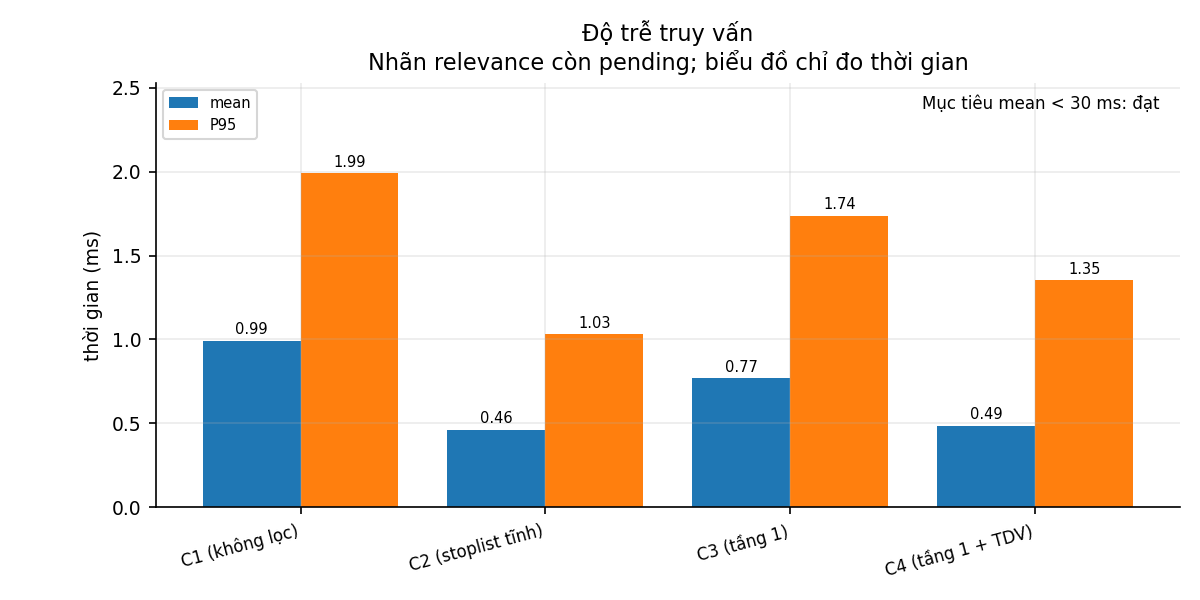
\includegraphics[width=.9\textwidth]{figures/fig_latency.png}\caption{Mean/P95 truy vấn BiMM.}\end{figure}

\begin{figure}[htbp]\centering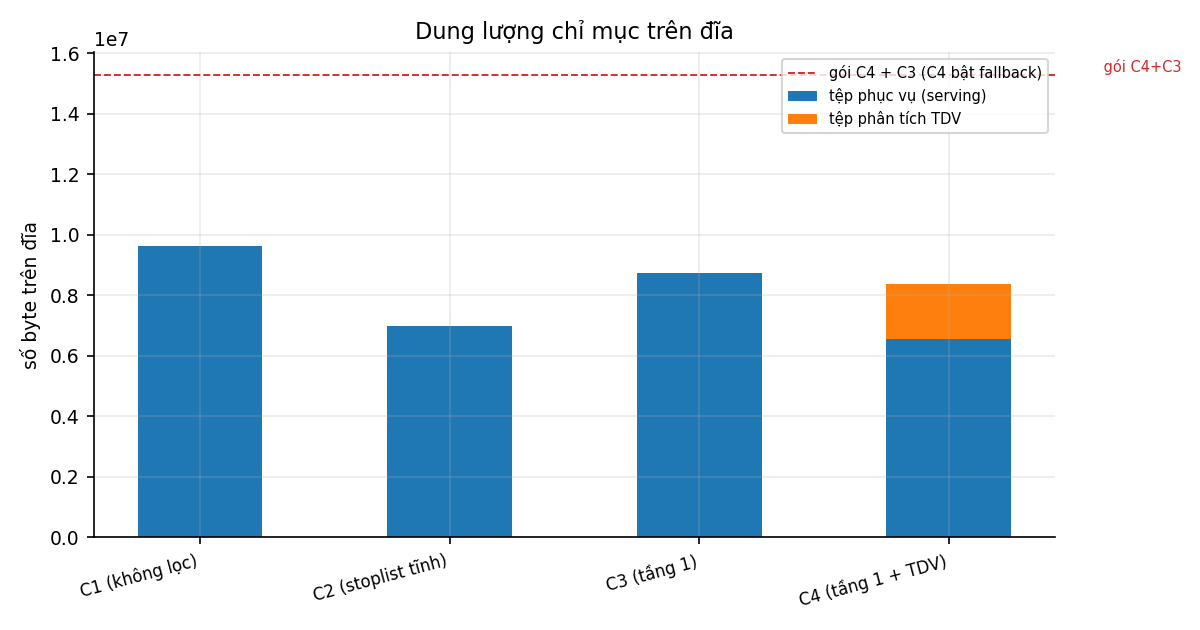
\includegraphics[width=.9\textwidth]{figures/fig_index_size.png}\caption{Dung lượng phục vụ, phân tích và gói fallback.}\end{figure}

\section{Thống kê TDV trên corpus đa lĩnh vực}

Mật độ gốc 0.03731830; chấm 31076 term, 666 điểm âm dưới dung sai. Bảo vệ 77 term theo whitelist/policy hợp từ; lọc thật 589 term. Thời gian TDV 12.641 giây, one-shot trên đủ 2.500 bài. Đây là tiêu chí hình học, không phải nhãn không liên quan ngữ nghĩa.

\begin{figure}[htbp]\centering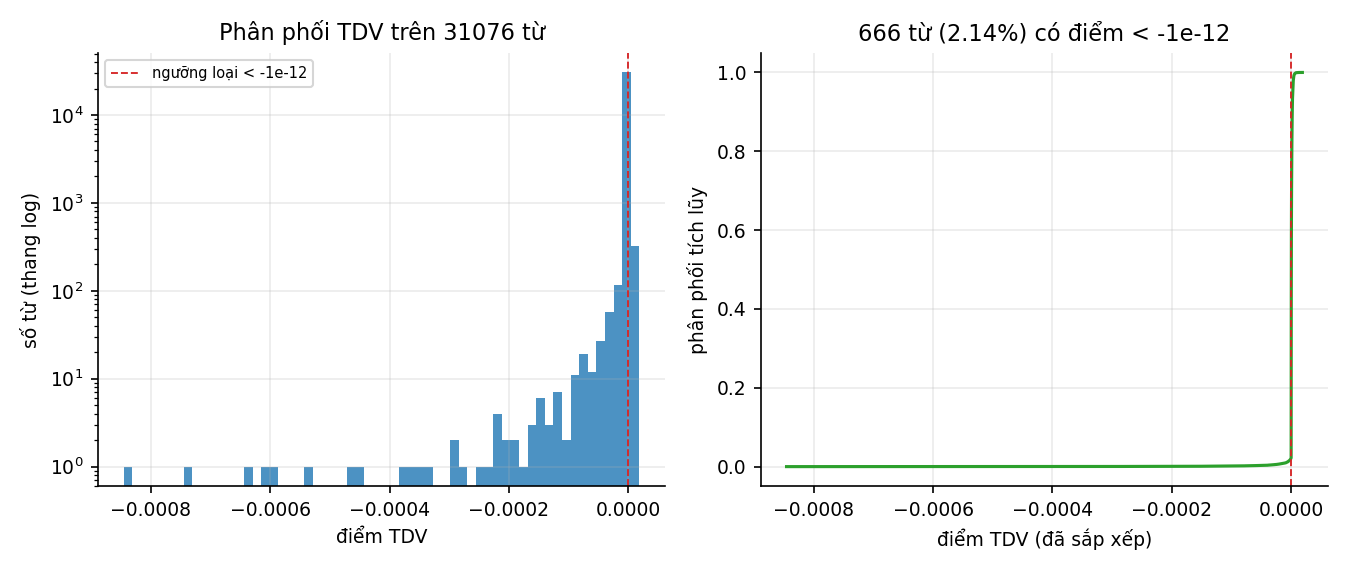
\includegraphics[width=.9\textwidth]{figures/fig_tdv_distribution.png}\caption{Phân bố TDV thực, không ép hình chữ U.}\end{figure}

\clearpage\section{Toàn bộ query và phân tích theo lĩnh vực}

\begin{longtable}{|l|p{.48\textwidth}|r|r|r|r|}
\hline
Query & Nội dung & C1 & C2 & C3 & C4 \\
\hline
\endhead
Q01 & lương tối thiểu & 0.153 & 0.091 & 0.188 & 0.089 \\
Q02 & biển cấm đỗ xe ô tô ở Hà Nội mất hiệu lực thì người dân đỗ xe ở đâu & 1.457 & 0.870 & 1.638 & 0.998 \\
Q03 & có nên tha thứ cho người vợ ngoại tình & 1.043 & 0.275 & 0.765 & 0.401 \\
Q04 & tâm sự gia đình & 0.198 & 0.244 & 0.162 & 0.031 \\
Q05 & nghiên cứu lõi băng để khám phá quy luật biến đổi khí hậu & 0.809 & 0.460 & 0.726 & 0.303 \\
Q06 & Trung Quốc xây trạm không gian và Nga phóng tàu lên ISS khác nhau như thế nào & 1.537 & 0.900 & 1.248 & 0.913 \\
Q07 & cổ phiếu & 0.066 & 0.055 & 0.107 & 0.079 \\
Q08 & lãi suất cơ bản và chính sách tiền tệ của Fed ảnh hưởng thị trường ra sao & 1.348 & 0.500 & 0.798 & 0.479 \\
Q09 & điều tra vụ biển thủ hơn 8,7 tỷ đồng cá độ bóng đá đã được xử lý ra sao & 1.596 & 0.502 & 1.377 & 0.379 \\
Q10 & đường dây chạy án trong vụ PMU18 & 0.833 & 0.289 & 0.362 & 0.238 \\
Q11 & ung thư & 0.064 & 0.087 & 0.074 & 0.102 \\
Q12 & mỡ máu cao nếu không điều trị có thể gây những biến chứng gì & 1.190 & 0.379 & 1.199 & 1.118 \\
Q13 & vì sao Mỹ vẫn chưa tìm thấy vũ khí cấm ở Iraq & 1.055 & 0.527 & 0.901 & 0.563 \\
Q14 & xác nhận danh tính hài cốt lính Mỹ mất tích trong Chiến tranh Triều Tiên & 1.037 & 0.697 & 0.653 & 0.457 \\
Q15 & vô địch & 0.091 & 0.117 & 0.144 & 0.019 \\
Q16 & Việt Nam đăng cai một vòng bảng Tiger Cup 2004 và các trận chung kết diễn ra thế nào & 1.723 & 0.814 & 1.499 & 1.388 \\
Q17 & cảnh nóng và trang phục hở trong phim truyền hình Việt Nam gây tranh luận như thế nào & 1.697 & 0.899 & 1.150 & 1.007 \\
Q18 & ca khúc và chương trình biểu diễn âm nhạc của nghệ sĩ & 1.182 & 0.464 & 0.502 & 0.275 \\
Q19 & virus máy tính đánh cắp mật khẩu Windows và cách phòng tránh & 1.224 & 0.412 & 0.643 & 0.351 \\
Q20 & dịch vụ phần mềm và thông tin di động được doanh nghiệp cung cấp cho khách hàng ra sao & 1.569 & 0.683 & 1.302 & 0.555 \\
\hline
\caption{Mean ms của toàn bộ 20 query.} \\
\end{longtable}

\begin{table}[htbp]
\centering
\begin{tabular}{|l|r|r|r|r|r|}
\hline
Lĩnh vực & Query & C1 & C2 & C3 & C4 \\
\hline
Chính trị – Xã hội & 2 & 0.805 & 0.481 & 0.913 & 0.543 \\
Đời sống & 2 & 0.621 & 0.259 & 0.464 & 0.216 \\
Khoa học & 2 & 1.173 & 0.680 & 0.987 & 0.608 \\
Kinh doanh & 2 & 0.707 & 0.277 & 0.452 & 0.279 \\
Pháp luật & 2 & 1.215 & 0.395 & 0.870 & 0.309 \\
Sức khỏe & 2 & 0.627 & 0.233 & 0.637 & 0.610 \\
Thế giới & 2 & 1.046 & 0.612 & 0.777 & 0.510 \\
Thể thao & 2 & 0.907 & 0.465 & 0.821 & 0.703 \\
Văn hóa & 2 & 1.440 & 0.681 & 0.826 & 0.641 \\
Vi tính & 2 & 1.397 & 0.548 & 0.973 & 0.453 \\
\hline
\end{tabular}
\caption{Mean ms theo 10 lĩnh vực; chỉ hai query/lĩnh vực.}
\end{table}

Mỗi lĩnh vực chỉ có hai query nên kết quả nhóm chưa đủ để suy rộng. Các bảng chất lượng toàn query/nhóm sẽ do evaluator xuất khi qrels đủ điều kiện, không thay dữ liệu thiếu bằng số 0.


\section{Định nghĩa chỉ số chất lượng và điều kiện công bố}

Cả bốn cấu hình dùng cùng corpus, query và qrels. Relevance là nhãn theo nội
dung của từng cặp query--document, không phải cùng lĩnh vực. Grade 0 là không
liên quan, grade 1 là liên quan một phần, grade 2 là đáp ứng trực tiếp;
grade lớn hơn 0 là relevant khi tính các chỉ số nhị phân.

Với $R_q$ là tập relevant đã biết của truy vấn $q$, $L_q^K$ là Top-$K$ kết quả:
\begin{align}
P@K &= \frac{|R_q\cap L_q^K|}{K},\\
Recall@K &= \frac{|R_q\cap L_q^K|}{|R_q|},\\
F1@K &= \frac{2\,P@K\,Recall@K}{P@K+Recall@K}.
\end{align}
Khi mẫu số bằng 0 quy ước kết quả bằng 0. Query không có relevant giữ điểm 0
trong bình quân macro và được đếm riêng; ranking rỗng cũng giữ 0, không loại khỏi
bình quân để làm đẹp kết quả. Mặc định $K=10$ cho Precision/Recall/F1/NDCG.

\begin{equation}
AP(q)=\frac{1}{|R_q|}\sum_{r=1}^{L}P@r\;rel(r),\qquad
MAP=\frac{1}{|Q|}\sum_{q\in Q}AP(q).
\end{equation}
$L$ là toàn ranking có sẵn (độ sâu mặc định bằng số tài liệu trong corpus).
Nếu cố ý cắt ranking phải ghi AP@depth, không gọi là MAP toàn ranking.
Document không có điểm dương không được bịa thành kết quả để đủ độ sâu.

\begin{equation}
DCG@K=\sum_{r=1}^{K}\frac{2^{grade(r)}-1}{\log_2(r+1)},\qquad
NDCG@K=\frac{DCG@K}{IDCG@K}.
\end{equation}
$IDCG$ lấy thứ tự grade lý tưởng từ qrels, không chỉ từ tài liệu đã trả về.
Nếu $IDCG=0$ thì NDCG bằng 0.

Bộ đánh giá chính thức kiểm tra schema, SHA256 corpus thực/manifest, SHA256
query, trạng thái nhãn, assessor và metadata preprocessing. Pending không được
tự diễn giải thành nhãn đã xác nhận. Khi chưa sẵn sàng, kết quả ghi
\texttt{unmeasured} và không xuất bảng điểm 0 như một phép đo chất lượng.
Các bảng theo query và 10 lĩnh vực được evaluator xuất khi qrels đủ điều kiện.

\section{Kiểm định tách từ và cấu trúc tra cứu}

Tập chuẩn bị cho M1 gồm 150 câu có nguồn từ corpus chính, 15 câu/lĩnh vực,
được lưu ở \texttt{data/gold/}. Gợi ý FMM/BMM/BiMM chỉ phục vụ gán nhãn;
không gọi output của thuật toán là gold. Người gán cần xác nhận phân đoạn,
assessor, nội dung chuẩn hóa và hash trước khi đo.

Đánh giá dùng khớp span từ trên cùng chuỗi âm tiết chuẩn hóa: một từ chỉ đúng
khi cả đầu và cuối span đều khớp. Precision là số span khớp chia span dự đoán,
Recall chia span gold, F1 là trung bình điều hòa. Không dùng tỷ lệ khớp ký tự
thay cho độ chính xác phân đoạn từ. Quy trình nhập nhãn phải từ chối phân đoạn
làm mất/thêm/đổi thứ tự âm tiết. Tệp hiện có 150/150 câu mang cờ xác nhận;
đường đánh giá chỉ được dùng làm kết luận sau khi nhãn gold được duyệt nội dung.
Rà soát bản gold hiện tại thấy 102 câu giữ nguyên toàn bộ gợi ý BiMM. Ít nhất
SG010, SG053 và SG089 có phân đoạn cần người gán xem lại; ví dụ SG010 ghép
``độc\_đáo\_để''. Sự trùng gợi ý không tự chứng minh nhãn sai,
nhưng số đo trên nhãn hiện có cần được kiểm tra độc lập trước khi coi là kết luận
cuối. Bảng F1 dưới đây được sinh lại từ kết quả đánh giá khớp bản gold đang dùng;
nếu thiếu hoặc lệch bản gold thì không được giữ số cũ.
\IfFileExists{segmentation_results.tex}{% Generated by python -m scripts.render_report; do not hand edit.

\textbf{Phân đoạn từ: số đo trên nhãn hiện có, tạm thời khi audit gold còn mở.} Word-span micro trên 150 câu; chỉ công bố là kết quả cuối sau khi duyệt các cặp nghi vấn.

\begin{table}[htbp]
\centering
\begin{tabular}{|l|r|r|r|}
\hline
Thuật toán & Precision & Recall & F1 \\
\hline
FMM & 0.9517 & 0.9643 & 0.9580 \\
BMM & 0.9561 & 0.9688 & 0.9624 \\
BiMM & 0.9561 & 0.9688 & 0.9624 \\
\hline
\end{tabular}
\caption{Word-span micro trên 150 câu gold hiện có; cần rà soát nhãn.}
\end{table}
}{\par\emph{Chưa có bảng F1 tách từ hợp lệ cho bản gold hiện tại.}}

Đối chứng Trie và Set phải dùng cùng từ điển, câu, cửa sổ và luật BiMM. Kiểm tra
output parity trước khi so tốc độ. Thời gian khởi tạo và bộ nhớ Python qua
\texttt{tracemalloc} tách khỏi thời gian tách câu; không gọi đây là toàn bộ RAM
tiến trình. Không mặc định Trie luôn nhanh hơn hash set.
Phép đo thật trên 150 câu mẫu và 100 bài đầu của corpus khóa (10 vòng lặp,
2 lượt warm-up) có 750 đối soát FMM/BMM/BiMM, không có token nào lệch.
Trên mẫu câu, mean FMM là 0,2328~ms (Trie) so với 0,1147~ms (Set), BiMM là
0,4557 so với 0,1958~ms; trên lát cắt corpus, BiMM là 6,5355 so với
2,6611~ms/bài. Như vậy bản Trie \emph{hiện tại} chậm hơn Set khoảng 2--2,5
lần trong hai workload này. Nguyên nhân triển khai là mỗi độ dài ứng viên lại
tra từ gốc Trie thay vì dùng một lượt dò tiền tố; đây không phải kết luận rằng
Trie nói chung chậm hơn. Đỉnh heap Python khi dựng Trie/Set lần lượt là
20.985.701/15.368.109 byte, không phải RSS. Chi tiết và dữ liệu gốc nằm trong
\texttt{results/lookup/trie\_vs\_set.json} và tài liệu benchmark kèm repo.

\section{Kiểm chứng triển khai}

\subsection{TF-IDF, Cosine và persistence}

Kiểm thử toán học dùng fixture tính tay và đối soát scikit-learn với cùng
analyzer/sublinear TF/smoothed IDF/L2, gồm từ lặp và token một ký tự.
Kiểm tra query rỗng, OOV, vector 0, stopword, hòa điểm, query dùng IDF corpus.
Kiểm thử save/load kiểm tra SHA256 artifact, source và tài nguyên; từ chối
tokenizer không thể kiểm chứng và nguồn bị thay đổi.

\texttt{explain()} phân rã bằng tích trọng số query/document đã L2; tổng phải
bằng điểm Cosine trong sai số số thực. Audit đầu-cuối đối chiếu từng kết quả
Top-10 của cả 20 query ở bốn cấu hình và kiểm tra nội dung pool với corpus khóa.

\subsection{TDV}

Đường tham chiếu độc lập dựng ma trận Cosine trực tiếp sau khi xóa từng chiều,
chuẩn hóa lại rồi tính mật độ. Đường nhanh dùng cấu trúc thưa và cập nhật tổng
vector chính xác. Kiểm thử gồm zero vector, một tài liệu, term xuất hiện mọi
tài liệu, dữ liệu ngẫu nhiên, và phản ví dụ cho cách xóa chiều mà không L2 lại.
Không sao chép kết quả tham chiếu làm output của đường tối ưu.

\subsection{Maximum Matching và giao diện}

FMM/BMM/BiMM được kiểm tra bằng từ điển fixture minh bạch, thứ tự trọng tài,
OOV xen kẽ từ đã biết và ranh giới dấu câu. Lead còn dùng oracle Set trực tiếp
độc lập trên từ điển/câu ngẫu nhiên; trace phải tái dựng đúng output khi sắp
terminal action theo vị trí, trong khi thứ tự bước BMM vẫn phản ánh quét lùi.
AppTest chạy mã Streamlit thật cho trang chủ, ba phương pháp, tầng 1, tìm kiếm,
explain, OOV và Analytics.

Báo cáo kiểm chứng đầy đủ và số test cuối nằm ở
\texttt{docs/integration\_status.md}; audit JSON ghi hash, số bài và sai số
phân rã Cosine. Fixture không được đưa vào bảng kết quả corpus chính.

\section{Giới hạn và kết luận}

Đường đánh giá đã tính chất lượng trên 669/669 cặp có cờ xác nhận. Các giá trị
MAP, P@10 và NDCG@10 trong bảng đầu chương là số đo trên tệp nhãn lúc chạy;
không diễn giải thứ hạng giữa các cấu hình là ưu thế có ý nghĩa thống kê hoặc
suy rộng sang kho ngữ liệu khác. Hai phiếu rà soát bằng AI đã liệt kê 37 cặp
qrels không trùng nhau; Team7 gửi quyết định cho cả 37 và sau đó sửa riêng
Q16/\texttt{vn\_f4f2b5ae9443c172} từ mức 2 xuống mức 1. Phép đo trong bảng
đã chạy lại trên qrels mới (SHA256 bắt đầu \texttt{697fafc7}); không dùng
CSV trước lần nhập. Nguồn chấm độc lập M1 vẫn chưa được xác minh, nên kết luận
ngữ nghĩa còn tạm thời dù cổng kỹ thuật đánh giá đã cho phép. Chi tiết nằm
trong biên bản \path{results/label_review_resolution.json}.
Tập query nhỏ (hai/lĩnh vực) và qrels pooling có thiên lệch theo các hệ thống
đóng góp; tài liệu relevant bị cả ba baseline bỏ sót không có nhãn, không có
hướng sai lệch cố định của MAP/Recall so với relevance đầy đủ.

Maximum Matching phụ thuộc từ điển, dễ nhập nhằng với tên riêng, từ mới và cụm
dài; từ điển rộng có cả thành ngữ không đồng nghĩa là phân đoạn tốt. Chính sách
chuẩn hóa bỏ số/URL/email và giữ chữ Latin vay mượn cần được cân nhắc khi đọc
query chuyên ngành. Bag-of-words giữ phủ định không có nghĩa đã suy luận đúng
ngữ nghĩa phủ định.

Số đo latency là warm process trên một máy, không phải cam kết độ trễ mọi máy
hay mọi kích thước corpus. Kết quả kích thước phải tách chỉ mục C4 thuần khỏi gói
C4+C3. Phần triển khai, tích hợp và phép tính đã chạy; kết luận chất lượng cuối
cần được cập nhật sau khi mẫu kiểm tra chéo và gold tách từ được duyệt.
}{
  \chapter{THỰC NGHIỆM VÀ ĐÁNH GIÁ}
  Nội dung thực nghiệm M2 chờ tệp chapter4.tex.
}

% Chương 5 — Kết luận. Nạp bằng % Chương 5 — Kết luận. Nạp bằng % Chương 5 — Kết luận. Nạp bằng \input{chapter5}. Chỉ dùng các gói đã khai báo.
\chapter{KẾT LUẬN VÀ HƯỚNG PHÁT TRIỂN}
\label{ch:ch5-ketluan}

\section{Kết quả đạt được}

Đồ án đã hoàn thành một hệ thống truy xuất văn bản tiếng Việt chạy hoàn toàn ngoại
tuyến, gồm ba tầng trách nhiệm rõ ràng. Tầng ngôn ngữ M1 thực hiện chuẩn hóa chuỗi,
tách từ theo so khớp cực đại trên từ điển Viet74K \cite{viet74k} và lọc từ dừng
tầng~1 kèm danh sách bảo vệ phủ định. Tầng truy xuất M2 biến dãy token thành chỉ
mục đảo, tính trọng số TF-IDF theo mô hình không gian vector \cite{salton1975vsm}
và xếp hạng bằng tương đồng cosin, đồng thời cài đặt độ đo Giá trị phân biệt từ
theo hướng tiếp cận của Salton và cộng sự \cite{salton1975theory} làm tầng lọc thứ
hai. Tầng tích hợp M3 cung cấp ứng dụng minh họa, hợp đồng API và bộ công cụ đóng
gói.

Bốn cấu hình thực nghiệm C1--C4 đã được dựng trên cùng một kho ngữ liệu gồm 2.500
bài thuộc 10 lĩnh vực và cùng một bộ 20 truy vấn: C1 không lọc, C2 lọc bằng danh
sách tĩnh, C3 lọc bằng hư từ tầng~1 của M1, và C4 lọc tầng~1 cộng thêm tầng~2 bằng
TDV. Các chỉ mục đã được dựng lại trên Maximum Matching chính thức của M1, với
metadata ghi rõ tokenizer, tài nguyên và hàm băm nguồn, nên so sánh giữa bốn cấu
hình là so sánh đúng một yếu tố: chiến lược lọc từ dừng.

\section{Những gì đã được kiểm chứng}

Phần tính toán cốt lõi đã được kiểm chứng bằng các đường tham chiếu độc lập, không
chỉ bằng các ca kiểm thử tự viết:

\begin{itemize}
  \item \textbf{TDV.} Đường tính nhanh trên cấu trúc thưa khớp với đường tham
        chiếu dựng ma trận cosin đầy đủ sau khi xóa từng chiều và tái chuẩn hóa,
        trong sai số số thực dưới $10^{-15}$. Bộ kiểm thử còn dựng sẵn một hàm mô
        phỏng ``cách làm sai'' (xóa chiều mà không tái chuẩn hóa) và khẳng định kết
        quả của engine khác kết quả sai đó, qua đó chứng minh tầm quan trọng của
        bước tái chuẩn hóa.
  \item \textbf{Chỉ số đánh giá.} Các định nghĩa $P@K$, $Recall@K$, $F1@K$, $AP$ và
        $NDCG@K$ được kiểm chứng bằng fixture tính tay; trọng số TF-IDF được đối
        soát với thư viện scikit-learn \cite{sklearn_tfidf} trên cùng cấu hình
        analyzer, sublinear TF, IDF làm mượt và chuẩn hóa L2.
  \item \textbf{Tách từ.} Ba phương pháp FMM/BMM/BiMM được kiểm chứng bằng từ điển
        fixture minh bạch, với quy tắc phân xử của BiMM được phát biểu tường minh.
        Vết thuật toán cho thấy ứng viên và quyết định tại từng bước; dãy token do
        \texttt{tokenize} trả về được kiểm riêng bằng fixture, không dùng các dòng
        ứng viên được đánh dấu của BMM để tái dựng kết quả.
  \item \textbf{Toàn vẹn dữ liệu.} Bộ đánh giá từ chối ghi kết quả chính thức khi
        hàm băm kho ngữ liệu, hàm băm tập truy vấn, trạng thái nhãn hoặc metadata
        tiền xử lý không đạt yêu cầu. Cơ chế khóa hàm băm tập truy vấn ngăn việc
        dùng nhầm nhãn cho một phiên bản truy vấn đã bị sửa.
  \item \textbf{Độ trễ và dung lượng.} Cả bốn cấu hình đã được đo độ trễ truy vấn và
        dung lượng chỉ mục trên máy cục bộ, với quy trình đo có bước khởi động làm
        nóng và có báo cáo theo từng truy vấn. Số đo chi tiết cùng trạng thái đạt
        hoặc không đạt mục tiêu được trình bày ở Chương~4.
\end{itemize}

\section{Những gì chưa đo được}

Báo cáo nêu rõ hai khoảng trống dữ liệu, và không thay thế chúng bằng kết luận định
tính:

\begin{enumerate}
  \item \textbf{Chỉ số chất lượng truy xuất chưa được đo.} Pool đánh giá có hàng
        trăm cặp ứng viên do ba đường cơ sở đóng góp, nhưng tại thời điểm viết
        \textbf{chưa có cặp nào được người gán xác nhận}; trạng thái nhãn là
        \texttt{pending\_human\_annotation}. Vì vậy bộ đánh giá ghi
        \texttt{metrics\_status = unmeasured} và cố ý không xuất bảng $P@K, R@K,
        F1@K, MAP, NDCG@K$. Không có kết luận nào về việc cấu hình nào cho chất
        lượng truy xuất tốt hơn, kể cả khi dung lượng chỉ mục của một cấu hình nhỏ
        hơn hay truy vấn của nó nhanh hơn.
  \item \textbf{Chất lượng tách từ chưa được đo.} Bộ mẫu 150 câu (15 câu mỗi lĩnh
        vực) rút từ kho ngữ liệu đã khóa vẫn ở trạng thái chờ người gán. Do đó
        không có chỉ số $F1$ tách từ nào cho cả ba phương pháp. Gợi ý của máy chỉ
        là công cụ hỗ trợ gán nhãn, không phải nhãn vàng.
\end{enumerate}

Việc giữ nguyên trạng thái ``chưa đo'' là một phần của kết quả: nó buộc mọi kết
luận về chất lượng phải chờ dữ liệu người, thay vì dựa vào các con số thời gian và
dung lượng vốn không phản ánh mức độ liên quan.

\section{Hạn chế}

Các hạn chế dưới đây cần được đọc kèm với các kết quả đã nêu:

\begin{itemize}
  \item \textbf{Phụ thuộc từ điển.} Chất lượng tách từ gắn chặt với từ điển đóng
        gói. Đổi từ điển thì mọi số đo tách từ phải được đo lại; từ điển rộng có
        thể chứa cả thành ngữ không đồng nghĩa với một phân đoạn từ tốt.
  \item \textbf{Lọc quá tay.} Cơ chế lọc theo tầng có thể loại cả những từ mang
        nghĩa với một số truy vấn cụ thể. Dung lượng nhỏ và truy vấn nhanh không
        chứng minh chất lượng tốt; vấn đề này chỉ giải quyết được khi có nhãn.
  \item \textbf{Phủ định ở mức túi từ.} Giữ lại từ phủ định tránh mất dấu hiệu phủ
        định ở mức từ vựng, nhưng mô hình túi từ vẫn không suy luận được ngữ nghĩa
        phủ định.
  \item \textbf{Quy mô đánh giá nhỏ và có thiên lệch.} Bộ truy vấn chỉ có 20 câu,
        khoảng hai câu mỗi lĩnh vực; pool được gộp từ chính các đường cơ sở nên có
        thể bỏ sót tài liệu liên quan không được đường nào trả về. Bộ mẫu tách từ
        150 câu, nếu chỉ một người gán, cũng không đo được đồng thuận giữa người gán.
  \item \textbf{Chi phí dự phòng.} Cơ chế dự phòng cho C4 khi mọi token truy vấn
        đều đã bị lọc đòi hỏi giữ thêm một chỉ mục C3. Việc giữ hai chỉ mục làm
        tổng dung lượng triển khai tăng lên, trái với mục tiêu giảm dung lượng của
        một chỉ mục đơn. Số liệu đo riêng chỉ mục C4 thuần và gói C4 cộng C3 được
        trình bày ở Chương~4.
  \item \textbf{Điều kiện đo độ trễ.} Độ trễ được đo trên tiến trình đã làm nóng
        trên một máy đơn, không phải cam kết về độ trễ trên mọi máy hay mọi kích
        thước kho ngữ liệu.
\end{itemize}

\section{Hướng phát triển}

Các bước tiếp theo được xác định theo thứ tự ưu tiên rõ ràng:

\begin{enumerate}
  \item Gán nhãn và xác nhận toàn bộ pool liên quan, sau đó chạy bộ đánh giá chính
        thức để có $P@K, R@K, F1@K, MAP, NDCG@K$ cho bốn cấu hình và cho từng lĩnh
        vực.
  \item Hoàn tất gán nhãn 150 câu mẫu tách từ, rồi chạy bộ đo khớp span để có $F1$
        cho FMM, BMM, BiMM.
  \item So sánh thêm với một bộ tách từ ngoài đã được công bố, trong điều kiện cho
        phép, để đặt kết quả của nhóm vào một mốc tham chiếu.
  \item Mở rộng bộ mẫu và số người gán để đo đồng thuận giữa người gán và để giảm
        độ dao động của chỉ số theo lĩnh vực.
  \item Nghiên cứu thay thế túi từ bằng một biểu diễn xử lý được phủ định ở mức
        ngữ nghĩa, và đánh giá lại tác động của việc bảo vệ guard.
\end{enumerate}

Cho tới khi các bước gán nhãn hoàn tất, kết luận đúng mực của đồ án là: hệ thống đã
hoàn tất về mặt triển khai và đã kiểm chứng được phần tính toán, thời gian và dung
lượng; phần kết luận về chất lượng truy xuất và chất lượng tách từ vẫn đang chờ
nhãn người.
. Chỉ dùng các gói đã khai báo.
\chapter{KẾT LUẬN VÀ HƯỚNG PHÁT TRIỂN}
\label{ch:ch5-ketluan}

\section{Kết quả đạt được}

Đồ án đã hoàn thành một hệ thống truy xuất văn bản tiếng Việt chạy hoàn toàn ngoại
tuyến, gồm ba tầng trách nhiệm rõ ràng. Tầng ngôn ngữ M1 thực hiện chuẩn hóa chuỗi,
tách từ theo so khớp cực đại trên từ điển Viet74K \cite{viet74k} và lọc từ dừng
tầng~1 kèm danh sách bảo vệ phủ định. Tầng truy xuất M2 biến dãy token thành chỉ
mục đảo, tính trọng số TF-IDF theo mô hình không gian vector \cite{salton1975vsm}
và xếp hạng bằng tương đồng cosin, đồng thời cài đặt độ đo Giá trị phân biệt từ
theo hướng tiếp cận của Salton và cộng sự \cite{salton1975theory} làm tầng lọc thứ
hai. Tầng tích hợp M3 cung cấp ứng dụng minh họa, hợp đồng API và bộ công cụ đóng
gói.

Bốn cấu hình thực nghiệm C1--C4 đã được dựng trên cùng một kho ngữ liệu gồm 2.500
bài thuộc 10 lĩnh vực và cùng một bộ 20 truy vấn: C1 không lọc, C2 lọc bằng danh
sách tĩnh, C3 lọc bằng hư từ tầng~1 của M1, và C4 lọc tầng~1 cộng thêm tầng~2 bằng
TDV. Các chỉ mục đã được dựng lại trên Maximum Matching chính thức của M1, với
metadata ghi rõ tokenizer, tài nguyên và hàm băm nguồn, nên so sánh giữa bốn cấu
hình là so sánh đúng một yếu tố: chiến lược lọc từ dừng.

\section{Những gì đã được kiểm chứng}

Phần tính toán cốt lõi đã được kiểm chứng bằng các đường tham chiếu độc lập, không
chỉ bằng các ca kiểm thử tự viết:

\begin{itemize}
  \item \textbf{TDV.} Đường tính nhanh trên cấu trúc thưa khớp với đường tham
        chiếu dựng ma trận cosin đầy đủ sau khi xóa từng chiều và tái chuẩn hóa,
        trong sai số số thực dưới $10^{-15}$. Bộ kiểm thử còn dựng sẵn một hàm mô
        phỏng ``cách làm sai'' (xóa chiều mà không tái chuẩn hóa) và khẳng định kết
        quả của engine khác kết quả sai đó, qua đó chứng minh tầm quan trọng của
        bước tái chuẩn hóa.
  \item \textbf{Chỉ số đánh giá.} Các định nghĩa $P@K$, $Recall@K$, $F1@K$, $AP$ và
        $NDCG@K$ được kiểm chứng bằng fixture tính tay; trọng số TF-IDF được đối
        soát với thư viện scikit-learn \cite{sklearn_tfidf} trên cùng cấu hình
        analyzer, sublinear TF, IDF làm mượt và chuẩn hóa L2.
  \item \textbf{Tách từ.} Ba phương pháp FMM/BMM/BiMM được kiểm chứng bằng từ điển
        fixture minh bạch, với quy tắc phân xử của BiMM được phát biểu tường minh.
        Vết thuật toán cho thấy ứng viên và quyết định tại từng bước; dãy token do
        \texttt{tokenize} trả về được kiểm riêng bằng fixture, không dùng các dòng
        ứng viên được đánh dấu của BMM để tái dựng kết quả.
  \item \textbf{Toàn vẹn dữ liệu.} Bộ đánh giá từ chối ghi kết quả chính thức khi
        hàm băm kho ngữ liệu, hàm băm tập truy vấn, trạng thái nhãn hoặc metadata
        tiền xử lý không đạt yêu cầu. Cơ chế khóa hàm băm tập truy vấn ngăn việc
        dùng nhầm nhãn cho một phiên bản truy vấn đã bị sửa.
  \item \textbf{Độ trễ và dung lượng.} Cả bốn cấu hình đã được đo độ trễ truy vấn và
        dung lượng chỉ mục trên máy cục bộ, với quy trình đo có bước khởi động làm
        nóng và có báo cáo theo từng truy vấn. Số đo chi tiết cùng trạng thái đạt
        hoặc không đạt mục tiêu được trình bày ở Chương~4.
\end{itemize}

\section{Những gì chưa đo được}

Báo cáo nêu rõ hai khoảng trống dữ liệu, và không thay thế chúng bằng kết luận định
tính:

\begin{enumerate}
  \item \textbf{Chỉ số chất lượng truy xuất chưa được đo.} Pool đánh giá có hàng
        trăm cặp ứng viên do ba đường cơ sở đóng góp, nhưng tại thời điểm viết
        \textbf{chưa có cặp nào được người gán xác nhận}; trạng thái nhãn là
        \texttt{pending\_human\_annotation}. Vì vậy bộ đánh giá ghi
        \texttt{metrics\_status = unmeasured} và cố ý không xuất bảng $P@K, R@K,
        F1@K, MAP, NDCG@K$. Không có kết luận nào về việc cấu hình nào cho chất
        lượng truy xuất tốt hơn, kể cả khi dung lượng chỉ mục của một cấu hình nhỏ
        hơn hay truy vấn của nó nhanh hơn.
  \item \textbf{Chất lượng tách từ chưa được đo.} Bộ mẫu 150 câu (15 câu mỗi lĩnh
        vực) rút từ kho ngữ liệu đã khóa vẫn ở trạng thái chờ người gán. Do đó
        không có chỉ số $F1$ tách từ nào cho cả ba phương pháp. Gợi ý của máy chỉ
        là công cụ hỗ trợ gán nhãn, không phải nhãn vàng.
\end{enumerate}

Việc giữ nguyên trạng thái ``chưa đo'' là một phần của kết quả: nó buộc mọi kết
luận về chất lượng phải chờ dữ liệu người, thay vì dựa vào các con số thời gian và
dung lượng vốn không phản ánh mức độ liên quan.

\section{Hạn chế}

Các hạn chế dưới đây cần được đọc kèm với các kết quả đã nêu:

\begin{itemize}
  \item \textbf{Phụ thuộc từ điển.} Chất lượng tách từ gắn chặt với từ điển đóng
        gói. Đổi từ điển thì mọi số đo tách từ phải được đo lại; từ điển rộng có
        thể chứa cả thành ngữ không đồng nghĩa với một phân đoạn từ tốt.
  \item \textbf{Lọc quá tay.} Cơ chế lọc theo tầng có thể loại cả những từ mang
        nghĩa với một số truy vấn cụ thể. Dung lượng nhỏ và truy vấn nhanh không
        chứng minh chất lượng tốt; vấn đề này chỉ giải quyết được khi có nhãn.
  \item \textbf{Phủ định ở mức túi từ.} Giữ lại từ phủ định tránh mất dấu hiệu phủ
        định ở mức từ vựng, nhưng mô hình túi từ vẫn không suy luận được ngữ nghĩa
        phủ định.
  \item \textbf{Quy mô đánh giá nhỏ và có thiên lệch.} Bộ truy vấn chỉ có 20 câu,
        khoảng hai câu mỗi lĩnh vực; pool được gộp từ chính các đường cơ sở nên có
        thể bỏ sót tài liệu liên quan không được đường nào trả về. Bộ mẫu tách từ
        150 câu, nếu chỉ một người gán, cũng không đo được đồng thuận giữa người gán.
  \item \textbf{Chi phí dự phòng.} Cơ chế dự phòng cho C4 khi mọi token truy vấn
        đều đã bị lọc đòi hỏi giữ thêm một chỉ mục C3. Việc giữ hai chỉ mục làm
        tổng dung lượng triển khai tăng lên, trái với mục tiêu giảm dung lượng của
        một chỉ mục đơn. Số liệu đo riêng chỉ mục C4 thuần và gói C4 cộng C3 được
        trình bày ở Chương~4.
  \item \textbf{Điều kiện đo độ trễ.} Độ trễ được đo trên tiến trình đã làm nóng
        trên một máy đơn, không phải cam kết về độ trễ trên mọi máy hay mọi kích
        thước kho ngữ liệu.
\end{itemize}

\section{Hướng phát triển}

Các bước tiếp theo được xác định theo thứ tự ưu tiên rõ ràng:

\begin{enumerate}
  \item Gán nhãn và xác nhận toàn bộ pool liên quan, sau đó chạy bộ đánh giá chính
        thức để có $P@K, R@K, F1@K, MAP, NDCG@K$ cho bốn cấu hình và cho từng lĩnh
        vực.
  \item Hoàn tất gán nhãn 150 câu mẫu tách từ, rồi chạy bộ đo khớp span để có $F1$
        cho FMM, BMM, BiMM.
  \item So sánh thêm với một bộ tách từ ngoài đã được công bố, trong điều kiện cho
        phép, để đặt kết quả của nhóm vào một mốc tham chiếu.
  \item Mở rộng bộ mẫu và số người gán để đo đồng thuận giữa người gán và để giảm
        độ dao động của chỉ số theo lĩnh vực.
  \item Nghiên cứu thay thế túi từ bằng một biểu diễn xử lý được phủ định ở mức
        ngữ nghĩa, và đánh giá lại tác động của việc bảo vệ guard.
\end{enumerate}

Cho tới khi các bước gán nhãn hoàn tất, kết luận đúng mực của đồ án là: hệ thống đã
hoàn tất về mặt triển khai và đã kiểm chứng được phần tính toán, thời gian và dung
lượng; phần kết luận về chất lượng truy xuất và chất lượng tách từ vẫn đang chờ
nhãn người.
. Chỉ dùng các gói đã khai báo.
\chapter{KẾT LUẬN VÀ HƯỚNG PHÁT TRIỂN}
\label{ch:ch5-ketluan}

\section{Kết quả đạt được}

Đồ án đã hoàn thành một hệ thống truy xuất văn bản tiếng Việt chạy hoàn toàn ngoại
tuyến, gồm ba tầng trách nhiệm rõ ràng. Tầng ngôn ngữ M1 thực hiện chuẩn hóa chuỗi,
tách từ theo so khớp cực đại trên từ điển Viet74K \cite{viet74k} và lọc từ dừng
tầng~1 kèm danh sách bảo vệ phủ định. Tầng truy xuất M2 biến dãy token thành chỉ
mục đảo, tính trọng số TF-IDF theo mô hình không gian vector \cite{salton1975vsm}
và xếp hạng bằng tương đồng cosin, đồng thời cài đặt độ đo Giá trị phân biệt từ
theo hướng tiếp cận của Salton và cộng sự \cite{salton1975theory} làm tầng lọc thứ
hai. Tầng tích hợp M3 cung cấp ứng dụng minh họa, hợp đồng API và bộ công cụ đóng
gói.

Bốn cấu hình thực nghiệm C1--C4 đã được dựng trên cùng một kho ngữ liệu gồm 2.500
bài thuộc 10 lĩnh vực và cùng một bộ 20 truy vấn: C1 không lọc, C2 lọc bằng danh
sách tĩnh, C3 lọc bằng hư từ tầng~1 của M1, và C4 lọc tầng~1 cộng thêm tầng~2 bằng
TDV. Các chỉ mục đã được dựng lại trên Maximum Matching chính thức của M1, với
metadata ghi rõ tokenizer, tài nguyên và hàm băm nguồn, nên so sánh giữa bốn cấu
hình là so sánh đúng một yếu tố: chiến lược lọc từ dừng.

\section{Những gì đã được kiểm chứng}

Phần tính toán cốt lõi đã được kiểm chứng bằng các đường tham chiếu độc lập, không
chỉ bằng các ca kiểm thử tự viết:

\begin{itemize}
  \item \textbf{TDV.} Đường tính nhanh trên cấu trúc thưa khớp với đường tham
        chiếu dựng ma trận cosin đầy đủ sau khi xóa từng chiều và tái chuẩn hóa,
        trong sai số số thực dưới $10^{-15}$. Bộ kiểm thử còn dựng sẵn một hàm mô
        phỏng ``cách làm sai'' (xóa chiều mà không tái chuẩn hóa) và khẳng định kết
        quả của engine khác kết quả sai đó, qua đó chứng minh tầm quan trọng của
        bước tái chuẩn hóa.
  \item \textbf{Chỉ số đánh giá.} Các định nghĩa $P@K$, $Recall@K$, $F1@K$, $AP$ và
        $NDCG@K$ được kiểm chứng bằng fixture tính tay; trọng số TF-IDF được đối
        soát với thư viện scikit-learn \cite{sklearn_tfidf} trên cùng cấu hình
        analyzer, sublinear TF, IDF làm mượt và chuẩn hóa L2.
  \item \textbf{Tách từ.} Ba phương pháp FMM/BMM/BiMM được kiểm chứng bằng từ điển
        fixture minh bạch, với quy tắc phân xử của BiMM được phát biểu tường minh.
        Vết thuật toán cho thấy ứng viên và quyết định tại từng bước; dãy token do
        \texttt{tokenize} trả về được kiểm riêng bằng fixture, không dùng các dòng
        ứng viên được đánh dấu của BMM để tái dựng kết quả.
  \item \textbf{Toàn vẹn dữ liệu.} Bộ đánh giá từ chối ghi kết quả chính thức khi
        hàm băm kho ngữ liệu, hàm băm tập truy vấn, trạng thái nhãn hoặc metadata
        tiền xử lý không đạt yêu cầu. Cơ chế khóa hàm băm tập truy vấn ngăn việc
        dùng nhầm nhãn cho một phiên bản truy vấn đã bị sửa.
  \item \textbf{Độ trễ và dung lượng.} Cả bốn cấu hình đã được đo độ trễ truy vấn và
        dung lượng chỉ mục trên máy cục bộ, với quy trình đo có bước khởi động làm
        nóng và có báo cáo theo từng truy vấn. Số đo chi tiết cùng trạng thái đạt
        hoặc không đạt mục tiêu được trình bày ở Chương~4.
\end{itemize}

\section{Những gì chưa đo được}

Báo cáo nêu rõ hai khoảng trống dữ liệu, và không thay thế chúng bằng kết luận định
tính:

\begin{enumerate}
  \item \textbf{Chỉ số chất lượng truy xuất chưa được đo.} Pool đánh giá có hàng
        trăm cặp ứng viên do ba đường cơ sở đóng góp, nhưng tại thời điểm viết
        \textbf{chưa có cặp nào được người gán xác nhận}; trạng thái nhãn là
        \texttt{pending\_human\_annotation}. Vì vậy bộ đánh giá ghi
        \texttt{metrics\_status = unmeasured} và cố ý không xuất bảng $P@K, R@K,
        F1@K, MAP, NDCG@K$. Không có kết luận nào về việc cấu hình nào cho chất
        lượng truy xuất tốt hơn, kể cả khi dung lượng chỉ mục của một cấu hình nhỏ
        hơn hay truy vấn của nó nhanh hơn.
  \item \textbf{Chất lượng tách từ chưa được đo.} Bộ mẫu 150 câu (15 câu mỗi lĩnh
        vực) rút từ kho ngữ liệu đã khóa vẫn ở trạng thái chờ người gán. Do đó
        không có chỉ số $F1$ tách từ nào cho cả ba phương pháp. Gợi ý của máy chỉ
        là công cụ hỗ trợ gán nhãn, không phải nhãn vàng.
\end{enumerate}

Việc giữ nguyên trạng thái ``chưa đo'' là một phần của kết quả: nó buộc mọi kết
luận về chất lượng phải chờ dữ liệu người, thay vì dựa vào các con số thời gian và
dung lượng vốn không phản ánh mức độ liên quan.

\section{Hạn chế}

Các hạn chế dưới đây cần được đọc kèm với các kết quả đã nêu:

\begin{itemize}
  \item \textbf{Phụ thuộc từ điển.} Chất lượng tách từ gắn chặt với từ điển đóng
        gói. Đổi từ điển thì mọi số đo tách từ phải được đo lại; từ điển rộng có
        thể chứa cả thành ngữ không đồng nghĩa với một phân đoạn từ tốt.
  \item \textbf{Lọc quá tay.} Cơ chế lọc theo tầng có thể loại cả những từ mang
        nghĩa với một số truy vấn cụ thể. Dung lượng nhỏ và truy vấn nhanh không
        chứng minh chất lượng tốt; vấn đề này chỉ giải quyết được khi có nhãn.
  \item \textbf{Phủ định ở mức túi từ.} Giữ lại từ phủ định tránh mất dấu hiệu phủ
        định ở mức từ vựng, nhưng mô hình túi từ vẫn không suy luận được ngữ nghĩa
        phủ định.
  \item \textbf{Quy mô đánh giá nhỏ và có thiên lệch.} Bộ truy vấn chỉ có 20 câu,
        khoảng hai câu mỗi lĩnh vực; pool được gộp từ chính các đường cơ sở nên có
        thể bỏ sót tài liệu liên quan không được đường nào trả về. Bộ mẫu tách từ
        150 câu, nếu chỉ một người gán, cũng không đo được đồng thuận giữa người gán.
  \item \textbf{Chi phí dự phòng.} Cơ chế dự phòng cho C4 khi mọi token truy vấn
        đều đã bị lọc đòi hỏi giữ thêm một chỉ mục C3. Việc giữ hai chỉ mục làm
        tổng dung lượng triển khai tăng lên, trái với mục tiêu giảm dung lượng của
        một chỉ mục đơn. Số liệu đo riêng chỉ mục C4 thuần và gói C4 cộng C3 được
        trình bày ở Chương~4.
  \item \textbf{Điều kiện đo độ trễ.} Độ trễ được đo trên tiến trình đã làm nóng
        trên một máy đơn, không phải cam kết về độ trễ trên mọi máy hay mọi kích
        thước kho ngữ liệu.
\end{itemize}

\section{Hướng phát triển}

Các bước tiếp theo được xác định theo thứ tự ưu tiên rõ ràng:

\begin{enumerate}
  \item Gán nhãn và xác nhận toàn bộ pool liên quan, sau đó chạy bộ đánh giá chính
        thức để có $P@K, R@K, F1@K, MAP, NDCG@K$ cho bốn cấu hình và cho từng lĩnh
        vực.
  \item Hoàn tất gán nhãn 150 câu mẫu tách từ, rồi chạy bộ đo khớp span để có $F1$
        cho FMM, BMM, BiMM.
  \item So sánh thêm với một bộ tách từ ngoài đã được công bố, trong điều kiện cho
        phép, để đặt kết quả của nhóm vào một mốc tham chiếu.
  \item Mở rộng bộ mẫu và số người gán để đo đồng thuận giữa người gán và để giảm
        độ dao động của chỉ số theo lĩnh vực.
  \item Nghiên cứu thay thế túi từ bằng một biểu diễn xử lý được phủ định ở mức
        ngữ nghĩa, và đánh giá lại tác động của việc bảo vệ guard.
\end{enumerate}

Cho tới khi các bước gán nhãn hoàn tất, kết luận đúng mực của đồ án là: hệ thống đã
hoàn tất về mặt triển khai và đã kiểm chứng được phần tính toán, thời gian và dung
lượng; phần kết luận về chất lượng truy xuất và chất lượng tách từ vẫn đang chờ
nhãn người.

% references.tex — Danh mục tài liệu tham khảo. Nạp bằng % references.tex — Danh mục tài liệu tham khảo. Nạp bằng % references.tex — Danh mục tài liệu tham khảo. Nạp bằng \input{references}.
% Chỉ liệt kê các nguồn đã kiểm chứng, có trong docs/academic_sources.md và
% trong phần xuất xứ dữ liệu của kho mã nguồn.
\renewcommand{\bibname}{TÀI LIỆU THAM KHẢO}
\begin{thebibliography}{9}

\bibitem{baigiang}
Bộ môn Cơ sở dữ liệu Đa phương tiện.
\textit{Bài tập nhóm -- D23CQCNHT01}, đề tài 8: tách từ, loại từ dừng, TF-IDF,
tương đồng cosin và đánh giá kết quả. Tài liệu môn học, trang~2.

\bibitem{giaotrinh}
\textit{Chương 3 -- Hệ thống truy vấn thông tin văn bản}. Bài giảng môn học.
Các khái niệm tài liệu, truy vấn, chỉ mục, độ liên quan (tr.~6--9), đặc trưng
(tr.~12--13), chỉ mục đảo (tr.~20--24) và tách từ, từ dừng, chuẩn hóa (tr.~26--28).

\bibitem{salton1975theory}
G. Salton, C. S. Yang, and C. T. Yu.
\newblock A theory of term importance in automatic text analysis.
\newblock \textit{Journal of the American Society for Information Science},
26(1):33--44, 1975.
\newblock DOI: \url{https://doi.org/10.1002/asi.4630260106}.

\bibitem{salton1975vsm}
G. Salton, A. Wong, and C. S. Yang.
\newblock A vector space model for automatic indexing.
\newblock \textit{Communications of the ACM}, 18(11):613--620, 1975.
\newblock DOI: \url{https://doi.org/10.1145/361219.361220}.

\bibitem{cornell1974}
G. Salton, C. S. Yang, and C. T. Yu.
\newblock \textit{A Theory of Term Importance in Automatic Text Analysis}.
\newblock Technical report, Cornell University, 1974.
\newblock \url{https://ecommons.cornell.edu/entities/publication/0f17b8d0-4e8d-43b7-81c7-363fe12a51b9}.

\bibitem{sklearn_tfidf}
scikit-learn developers.
\newblock \texttt{TfidfTransformer} -- scikit-learn documentation.
\newblock \url{https://scikit-learn.org/stable/modules/generated/sklearn.feature_extraction.text.TfidfTransformer.html}.
\newblock Truy cập năm 2026. Dùng để đối soát cấu hình
\texttt{sublinear\_tf=True}, \texttt{smooth\_idf=True}, \texttt{norm='l2'}.

\bibitem{viet74k}
duyet.
\newblock \textit{Vietnamese wordlist (Viet74K)}, giấy phép GPL-2.0.
\newblock Kho mã nguồn mở trên GitHub:
\url{https://github.com/duyet/vietnamese-wordlist}.
\newblock Bản dùng trong đồ án được ghim ở commit
\texttt{688b0953c8cdb21ee090ce80b83cefdb052fe2cd}; từ điển đã làm sạch còn 69.858
mục.

\bibitem{static_stopwords}
Bản chụp danh sách từ dừng tiếng Việt (giấy phép MIT), dùng cho cấu hình C2.
\newblock Xuất xứ, phiên bản, số mục và thông báo giấy phép ghi trong
\texttt{resources/static\_stopwords\_source.md}.

\end{thebibliography}
.
% Chỉ liệt kê các nguồn đã kiểm chứng, có trong docs/academic_sources.md và
% trong phần xuất xứ dữ liệu của kho mã nguồn.
\renewcommand{\bibname}{TÀI LIỆU THAM KHẢO}
\begin{thebibliography}{9}

\bibitem{baigiang}
Bộ môn Cơ sở dữ liệu Đa phương tiện.
\textit{Bài tập nhóm -- D23CQCNHT01}, đề tài 8: tách từ, loại từ dừng, TF-IDF,
tương đồng cosin và đánh giá kết quả. Tài liệu môn học, trang~2.

\bibitem{giaotrinh}
\textit{Chương 3 -- Hệ thống truy vấn thông tin văn bản}. Bài giảng môn học.
Các khái niệm tài liệu, truy vấn, chỉ mục, độ liên quan (tr.~6--9), đặc trưng
(tr.~12--13), chỉ mục đảo (tr.~20--24) và tách từ, từ dừng, chuẩn hóa (tr.~26--28).

\bibitem{salton1975theory}
G. Salton, C. S. Yang, and C. T. Yu.
\newblock A theory of term importance in automatic text analysis.
\newblock \textit{Journal of the American Society for Information Science},
26(1):33--44, 1975.
\newblock DOI: \url{https://doi.org/10.1002/asi.4630260106}.

\bibitem{salton1975vsm}
G. Salton, A. Wong, and C. S. Yang.
\newblock A vector space model for automatic indexing.
\newblock \textit{Communications of the ACM}, 18(11):613--620, 1975.
\newblock DOI: \url{https://doi.org/10.1145/361219.361220}.

\bibitem{cornell1974}
G. Salton, C. S. Yang, and C. T. Yu.
\newblock \textit{A Theory of Term Importance in Automatic Text Analysis}.
\newblock Technical report, Cornell University, 1974.
\newblock \url{https://ecommons.cornell.edu/entities/publication/0f17b8d0-4e8d-43b7-81c7-363fe12a51b9}.

\bibitem{sklearn_tfidf}
scikit-learn developers.
\newblock \texttt{TfidfTransformer} -- scikit-learn documentation.
\newblock \url{https://scikit-learn.org/stable/modules/generated/sklearn.feature_extraction.text.TfidfTransformer.html}.
\newblock Truy cập năm 2026. Dùng để đối soát cấu hình
\texttt{sublinear\_tf=True}, \texttt{smooth\_idf=True}, \texttt{norm='l2'}.

\bibitem{viet74k}
duyet.
\newblock \textit{Vietnamese wordlist (Viet74K)}, giấy phép GPL-2.0.
\newblock Kho mã nguồn mở trên GitHub:
\url{https://github.com/duyet/vietnamese-wordlist}.
\newblock Bản dùng trong đồ án được ghim ở commit
\texttt{688b0953c8cdb21ee090ce80b83cefdb052fe2cd}; từ điển đã làm sạch còn 69.858
mục.

\bibitem{static_stopwords}
Bản chụp danh sách từ dừng tiếng Việt (giấy phép MIT), dùng cho cấu hình C2.
\newblock Xuất xứ, phiên bản, số mục và thông báo giấy phép ghi trong
\texttt{resources/static\_stopwords\_source.md}.

\end{thebibliography}
.
% Chỉ liệt kê các nguồn đã kiểm chứng, có trong docs/academic_sources.md và
% trong phần xuất xứ dữ liệu của kho mã nguồn.
\renewcommand{\bibname}{TÀI LIỆU THAM KHẢO}
\begin{thebibliography}{9}

\bibitem{baigiang}
Bộ môn Cơ sở dữ liệu Đa phương tiện.
\textit{Bài tập nhóm -- D23CQCNHT01}, đề tài 8: tách từ, loại từ dừng, TF-IDF,
tương đồng cosin và đánh giá kết quả. Tài liệu môn học, trang~2.

\bibitem{giaotrinh}
\textit{Chương 3 -- Hệ thống truy vấn thông tin văn bản}. Bài giảng môn học.
Các khái niệm tài liệu, truy vấn, chỉ mục, độ liên quan (tr.~6--9), đặc trưng
(tr.~12--13), chỉ mục đảo (tr.~20--24) và tách từ, từ dừng, chuẩn hóa (tr.~26--28).

\bibitem{salton1975theory}
G. Salton, C. S. Yang, and C. T. Yu.
\newblock A theory of term importance in automatic text analysis.
\newblock \textit{Journal of the American Society for Information Science},
26(1):33--44, 1975.
\newblock DOI: \url{https://doi.org/10.1002/asi.4630260106}.

\bibitem{salton1975vsm}
G. Salton, A. Wong, and C. S. Yang.
\newblock A vector space model for automatic indexing.
\newblock \textit{Communications of the ACM}, 18(11):613--620, 1975.
\newblock DOI: \url{https://doi.org/10.1145/361219.361220}.

\bibitem{cornell1974}
G. Salton, C. S. Yang, and C. T. Yu.
\newblock \textit{A Theory of Term Importance in Automatic Text Analysis}.
\newblock Technical report, Cornell University, 1974.
\newblock \url{https://ecommons.cornell.edu/entities/publication/0f17b8d0-4e8d-43b7-81c7-363fe12a51b9}.

\bibitem{sklearn_tfidf}
scikit-learn developers.
\newblock \texttt{TfidfTransformer} -- scikit-learn documentation.
\newblock \url{https://scikit-learn.org/stable/modules/generated/sklearn.feature_extraction.text.TfidfTransformer.html}.
\newblock Truy cập năm 2026. Dùng để đối soát cấu hình
\texttt{sublinear\_tf=True}, \texttt{smooth\_idf=True}, \texttt{norm='l2'}.

\bibitem{viet74k}
duyet.
\newblock \textit{Vietnamese wordlist (Viet74K)}, giấy phép GPL-2.0.
\newblock Kho mã nguồn mở trên GitHub:
\url{https://github.com/duyet/vietnamese-wordlist}.
\newblock Bản dùng trong đồ án được ghim ở commit
\texttt{688b0953c8cdb21ee090ce80b83cefdb052fe2cd}; từ điển đã làm sạch còn 69.858
mục.

\bibitem{static_stopwords}
Bản chụp danh sách từ dừng tiếng Việt (giấy phép MIT), dùng cho cấu hình C2.
\newblock Xuất xứ, phiên bản, số mục và thông báo giấy phép ghi trong
\texttt{resources/static\_stopwords\_source.md}.

\end{thebibliography}


\end{document}
